\documentclass[a4paper,12pt]{article}
\usepackage[utf8]{inputenc}
\usepackage[T1]{fontenc}
\usepackage[english, spanish]{babel}
\usepackage{hyperref}
\usepackage{eurosym}
\usepackage{amsmath}
\usepackage{amsfonts}
\usepackage{amssymb}
\usepackage{multirow}
\usepackage{flafter}
\usepackage{wrapfig}
% \usepackage{makeidx}
\usepackage{graphicx}
\usepackage{fancyhdr}
\usepackage{float}
\usepackage{upgreek}
\usepackage[table]{xcolor}
\definecolor{azulUC3M}{RGB}{0,6,124}
\definecolor{rojoUC3M}{RGB}{186,50,50}
\definecolor{verdeUC3M}{RGB}{86,204,86}
\definecolor{white}{RGB}{255,255,255}
\definecolor{gray97}{gray}{.97}
\definecolor{gray90}{gray}{.90}
\definecolor{gray75}{gray}{.75}
\definecolor{gray45}{gray}{.45}
\usepackage{colortbl}
\setlength\arrayrulewidth{1pt}

% Define the Use Case table with UC3M colors

\newenvironment{uc3m-table}[2]
% Header of the table
{\def\tableID{#1}
 \def\tableCaption{#2}

 \begin{table}[!htbp]
   \centering
   \rowcolors{2}{gray90}{white}
   
   \begin{tabular}{
     !{\color{azulUC3M}\vline} p{3cm}
     !{\color{azulUC3M}\vline} p{10cm}
     !{\color{azulUC3M}\vline}}
     \arrayrulecolor{azulUC3M}
     \rowcolor{azulUC3M}
     
     \multicolumn{1}{l !{\color{white}\vline}}
     {\color{white}{\texttt{ID}}}
     & \multicolumn{1}{l}
       {\color{white}{\texttt{#1}}} \\ }
% Footer of the table
{ \hline
  \end{tabular}
  \caption{\tableCaption}
  \label{\tableID}
\end{table} }

\usepackage{caption}
% \DeclareCaptionFont{white}{\color{white}}
% \DeclareCaptionFormat{listing}{\colorbox{azulUC3M}{\parbox{\textwidth}{#1#2#3}}}
% \captionsetup[lstlisting]{format=listing,labelfont=white,textfont=white}
\usepackage{rotating}
\usepackage{pdfpages}

\usepackage{listings}
\lstset{ frame=Ltb,
     framerule=0pt,
     %aboveskip=0.5cm,
     framextopmargin=3pt,
     framexbottommargin=3pt,
     framexleftmargin=0.2cm,
     xrightmargin=-0.7cm,
     xleftmargin=-0.5cm,
     belowcaptionskip=0.5cm,
     framesep=0pt,
     rulesep=0.2pt,
     backgroundcolor=\color{gray97},
     rulesepcolor=\color{black},
     %
     stringstyle=\ttfamily,
     showstringspaces = false,
     basicstyle=\fontsize{9pt}{12pt}\ttfamily,
     commentstyle=\color{gray45},
     keywordstyle=\bfseries,
     %
     breaklines=true,
     literate= {<lambda>}{$\lambda$}1 {²}{{\textsuperscript{2}}}1 {µ}{$\upmu$}1
   }

   \lstdefinestyle{haskell}{
     language=Haskell,
     numbers=left,
     numbersep=15pt,
     numberstyle=\tiny,
     numberfirstline=false,
   }

   \lstdefinestyle{shell}{
     escapeinside=\{\}
   }


\lstnewenvironment{listing}[1][]
{\lstset{#1}\pagebreak[0]}{\pagebreak[0]}

\usepackage[top=2cm]{geometry}
\pretolerance=2000
\tolerance=3000

\usepackage{pgfplots}
\usepackage{pgfgantt}

\pgfplotscreateplotcyclelist{list}{%
  {color=azulUC3M, fill=azulUC3M},
  {color=rojoUC3M, fill=rojoUC3M},
  {color=verdeUC3M, fill=verdeUC3M}
}

\usepackage{titlesec}
\usepackage[titletoc,toc,title]{appendix}

\begin{document}
\selectlanguage{english}

\begin{titlepage}
  \begin{sffamily}
  \color{azulUC3M}
  \begin{center}
    % \vspace*{-1cm}
    \begin{figure}[htb]
      \begin{center}
        \vspace*{0.6cm}
        
\includegraphics[width=15cm]{img/Portada_Logo.png}
        \vspace*{1.6cm}
      \end{center}
    \end{figure}
    
  \begin{Large}
    Bachelor's Degree in Computer Science \& Engineering\\
  \end{Large}
  
  \begin{LARGE}
    2016/2017 \\
    \vspace*{2cm}
    \textsl{Bachelor Thesis}\\
  \end{LARGE}
    
    \begin{huge}
      \textbf{Agis: Heuristic Search Library \& Framework in Haskell} \\
      \rule{80mm}{0.1mm}\\
      \vspace*{1cm}
      Diego Vicente Martín\\
    \end{huge}
    
    \vspace*{1cm}
    \begin{Large}
      Supervisor\\
      Carlos Linares López\\
      Leganés, October 16th 2017\\
    \end{Large}
  \end{center}
  \vspace*{4cm}
  \color{black}

  \begin{wrapfigure}{l}{0.2\textwidth}
    \vspace{-0.7cm}
    
\includegraphics[width=3cm]{img/creativecommons.png}
  \end{wrapfigure}


  This work is licensed under a Creative Commons \\
  \textbf{Attribution - NonCommercial - NoDerivatives}\\
  
\end{sffamily}
\end{titlepage}


\pagestyle{fancy}
\fancyhead{} % Clear all header fields
\setlength\headheight{21.2pt}
\lhead{\hspace*{-0.3cm}\raisebox{-0.3\height}{
    
\includegraphics[scale=0.44]{img/Portada_Logo.png}}}
\rhead{\color{azulUC3M} \texttt{Agis}: Heuristic Search in Haskell}

% \renewcommand{\tablename}{\textbf{Tabla}}
% \renewcommand{\figurename}{\textbf{Figura}}
% \renewcommand{\listtablename}{Índice de tablas}

\newpage

\tableofcontents

\newpage

\listoftables

\listoffigures

\lstlistoflistings

%Para imagenes
%\begin{figure}[H]
%\centering
%\includegraphics[scale=0.8]{imagenes/*.png}
%\caption{}
%\end{figure}

\newpage

% English summary
\vspace*{\fill}

\selectlanguage{english}
\begin{abstract}

There are currently few experiments that try to perform heuristic search in
Haskell, even though the language provides a clean and modular syntax
that can be specially useful for educational or research purposes in the field.
Furthermore, functional programming provides a inherently concurrent way of
writing code, which results in trivial parallelism using compiler flags. Also,
due to the particular constraints imposed by the language, it is specially
interesting to create a library of algorithms that solves the $k$ best paths
problem. Taking into account that it can be detrimental to the overall
performance, the language's nature allows the framework to return a list (that
can theoretically be as long as infinite) containing all the solutions in the
problem space, and use its lazy evaluation to only compute the $k$ solutions
asked by the user, without any kind of code modification.\\

The aforementioned reasons are found as a motivation for developing a framework
in Haskell, that allows the user to perform searches, as well as designing
different algorithms and test them along with the ones provided for comparison.
Haskell's strong type system let us declare a set of types used by the library,
declaring all needed constraints in them and ensuring that if the code provided
by the user type checks the code will most likely behave as expected by the
user.\\

This thesis details all the steps that were needed in the process: from a
software engineering approach to the design, to the generation of all needed
artifacts to ensure the quality and intuition about the library; including the
implementation step and all the reasoning behind it, and all formal
verification of the models used in the library. The testing process also
contains all the performance checks along with several low-level profile tests
to spot a space leak in the library. All the organizational, legal and
socioeconomic details of the project are also included in the document, along
with an appendix containing all the generated documentation of the framework.\\

The result is \texttt{agis}: a Haskell package that lets the user include in
their own code a set of types to model and solve heuristic problems; design
modular heuristic search algorithms (using intermediate functions provided by
the library) or write them from scratch (using the types provided by the
library) and be able to run them in several search domains provided in the
framework or run several benchmarks using a \texttt{criterion} interface.\\
\end{abstract}

\vspace*{\fill}

\newpage

% Spanish summary
\vspace*{\fill}

\selectlanguage{spanish}
\begin{abstract}

Actualmente existen pocos ejemplos de búsqueda heurística en Haskell, a pesar
de que el lenguaje ofrece una sintaxis modular y limpiar que lo hace
especialmente interesante para fines educativos o de investigación en este
campo. Además, la programación funcional ofrece una forma de escribir código
intrínsecamente concurrente, lo que hace código de Haskell trivialmente
paralelizable (tan solo es necesario activar ciertas opciones propuestas por el
compilador). Además de todo ello, las restricciones impuestas por el lenguaje
hacen una opción especialmente interesante que los algoritmos incluídos en la
librería no tengan un comportamiento clásico, sino que resuelvan a su vez el
problema de las $k$ mejores soluciones: el algoritmo puede devolver una lista
con todas las soluciones incluídas en el espacio de búsqueda (que puede ser
infinita), y usar la evaluación perezosa del lenguaje para solo calcular las
que el usuario realmente pida, sin ninguna modificación de código ni problema a
la hora de evaluar dicha lista.\\

Todas estas razones sirven de motivación para el desarrollo de un framework en
Haskell, que permita al usuario tanto ejecutar búsquedas como diseñar distintos
algoritmos y compararlos con otros ya existentes. El sistema de tipos de
Haskell permite a la librería declarar un conjunto de tipos para que sean
usados por el usuario a la hora de modelar problemas o diseñar algoritmos y
asegurar de esta manera que si el código compila, es muy probable que el
comportamiento del código sea el esperado.\\

En este trabajo se recogen todos los pasos que se han seguido en este proceso:
desde un diseño a nivel de ingeniería de software hasta la generación de todos
los artefactos necesarios para asegurar un correcto diseño de la librería, para
pasar a la implementación de dicho diseño. Esta implementación incluye todas
las justificaciones necesarias así como la verificación formal de los modelos
que así lo requiren. Se incluye una sección que define todas las pruebas
realizadas que incluyen la medición de tiempos y recursos, así como varias
pruebas de bajo nivel realizadas para encontrar el origen de una pérdida de
espacio y desempeño encontrada en la librería. Todos los los detalles
organizativos, legales y socioeconómicos se encuentran recogidos en este
documento, así como la documentación generada por la librería en un apéndice a
este.\\

El resultado del trabajo es \texttt{agis}: un paquete de Haskell que permite al
usuario incluir en su propio código un conjunto de tipos para modelar problemas
y resolverlos usando distintos algoritmos de búsqueda, diseñar algoritmos de
búsqueda modulares (usando funciones intermedias proporcionadas por el
framework) o implementar uno de cero (usando los tipos de la librería), y ser
así capaz de correrlos en distintos dominios de búsqueda incluidos en el
framework o correr distintos benchmarks con la interfaz proporcionada al
paquete \texttt{criterion}.\\
\end{abstract}

\vspace*{\fill}
\newpage


\selectlanguage{english}

\vspace*{4cm}

\section*{\centering{Acknowledgement}}

Thanks to Carlos Linares López, the supervisor of this thesis, for his
guideance. Without his trust in my own judgement and work, this thesis would
have never become what it came to be.\\

\selectlanguage{spanish}

Gracias a mis padres, por su apoyo y dedicación a lo largo de toda mi
educación. Este trabajo es tan vuestro como mío, aunque sé que siempre
pensásteis que me quedaría ciego de tanto mirar la pantalla antes de
terminar de escribirlo.\\

\vspace{1cm}

\selectlanguage{english}

\centerline{\emph{With a little help of my friends.}}

\newpage

%%% Local Variables:
%%% TeX-master: "tfg"
%%% End:
\section{Introduction}

The functional programming paradigm is nowadays an upward trend
\cite{ford-2013-ibm}, whose popularity can be traced to the several advantages
it offers: an arguably easier way of reasoning about its concepts, the use of
high-level abstractions that can be used for both reducing the workload on the
developers and including optimizations in the compiled code, or the fact that
its characteristics and principles make the fact of turning purely functional
code into concurrent code a trivial task \cite{hammond-2012-parallel}. This is
done by radically stripping the side effects from the code and keeping the
state of the machine immutable, or more recently, by isolating them and keeping
the referential transparency intact through as much as possible of the code base.\\

This trend is present in new languages being developed with the functional
paradigm: for instance, Scala \cite{scala} is a functional, strongly-typed
language based on the Java virtual machine, which makes it able to be used for
Android applications development. Another interesting example is Elm
\cite{elm}, which compiles to HTML, CSS and Javascript allowing functional web
development. But not only new languages are being inspired by functional
programming: long-established languages are also introducing functional
concepts such as map-reduce, folds, higher-order or anonymous functions into
traditional workflows. Some examples of this include Java \cite{java8},
C++ \cite{cpp-lambdas, cpp-high-level} or Python \cite{python-mrs}.\\

Arguably, the flagship language of the pure functional paradigm is Haskell
\cite{haskell-98}. Among its main features we can highlight the fact that it is
purely functional (and allows complete referential transparency by isolating
the side effects), lazy (contrary to strict evaluation, laziness implies that
only the required results are computed among all definitions), strongly and
statically typed (all types are checked at compile time) and provides a great
set of abstractions that can be compiled into concurrent code. This
particularities have placed on Haskell the stigma of being an academic
language, with hardly any practical use on real life; a stigma that the
community has worked exhaustively to get rid of.\\

Ironically enough, some Computer Science fields seem like unexplored territory
in Haskell. For example, a quick query on how many Haskell packages are
available on the most popular Haskell package manager related to heuristic
search returns a scarce set of algorithms, with different specifications and
barely any cohesion between them. That makes the task of studying the behavior
of different search algorithms in functional programming too much of a hassle,
compared to other languages with solid developed frameworks.\\

Out of this necessity the idea of \emph{Agis} is born: a full-fledged,
functional heuristic search framework. Agis not only provides a heuristic
search library with well known algorithms, but also the building blocks used to
implement them and a suite of different interfaces to performance and
automation tools for Haskell. The library is divided in two different flavors:
\texttt{Search.Pure}, which provides a set of completely pure functional
algorithms implemented and ready to be used; and \texttt{Search.Monadic}, which
adds a new layer of complexity using a monad that wraps the search. This causes
a time and space overhead with the advantage of being able to gather run-time
statistics, that can be used for educational, algorithm design or research
purposes. 

\newpage

%%% Local Variables:
%%% TeX-master: "tfg"
%%% End:

\section{State of the Art}

Before the main matter of the thesis, it is important to expose the current
state of the art, to check if the previous research done in the topics
related to this project. First, the section will sum up the current state of
the art in the algorithms that will be used by the thesis, as well as all
naming several libraries currently used for that purpose. Last, this section
will provide a basic state of the language to be used, Haskell; that will also
serve as a motivation for why to develop the project using this tool.\\

\subsection{Heuristic Search}

Heuristic Search is a problem solving method that belongs to Artificial
Intelligence \cite{rusell-2003-aima} used in robotics, pathfinding, computer
gaming among other fields. We can distinguish two types of heuristic search
algorithms: uninformed algorithms, which do not use a heuristic function and
perform a brute-force search; and informed algorithms, which use a heuristic
function to provide better performance than the aforementioned brute-force
algorithms.\\

\subsubsection{Uninformed Algorithms}

\subsubsection{Informed Algorithms}

\subsubsection{Libraries}

Due to being more appropriate for the performance that is in general desired,
we can find that the most amount of work on Heuristic Search is done in
imperative, fast languages like C++ or Java.\\

In C++, we can find full search frameworks like \emph{HOG2} \cite{hog2},
\emph{Research code for heuristic search} \cite{cpp-search} or \emph{The
  Heuristic Search Research Framework} \cite{goldenberg-2017-framework}. All
these frameworks offer a full set of algorithms and procedures to override the
default implementations (such as cost, heuristic or expansion functions) in
order to adapt the library's behavior to the problem at hand. Also, these
frameworks offer visual representations options; a feature which is indeed the
main goal in the case of \emph{The Heuristic Search Research Framework}, that
offers a general visualization of algorithm behavior instead of domain specific
ones. On the other hand, in Java we can find similar projects like
\emph{Combinatorial Search for Java} \cite{cs4j} or \emph{AIMA}
\cite{java-aima}.\\

Trying to find similar projects in functional languages is more complicated
than that. However, one can find interesting projects like \emph{AIMA} written
in Common Lisp \cite{lisp-aima} or even a complete search framework written in
OCaml \cite{ocaml-search}. In Haskell, however, projects of this size are
nowhere to be found: All the algorithms are distributed in individual packages
with completely different implementations, as well as the data structures used
to perform the search.


\subsection{Haskell}

Haskell's first version was released in 1990 after the efforts of a committee
in FPCA '87 for creating an open standard for a ``non-strict, purely functional
language'' \cite{haskell-history}. Haskell's main features have remain patent
in the language, but constantly evolving: the language's main pillars are
\cite{haskell-98, haskell-2010}:

\begin{enumerate}
\item \textbf{Strong and statically typed}: the types are checked at compile
  time. That makes the run-time be sure that every function will get as
  parameter the expected object, making it more robust. However, no explicit
  type declaration is needed (although it is usually considered a good
  practice); types can be inferred most of the times by the compiler.
\item \textbf{Purely functional}: this type system is what allows Haskell to be
  purely functional. For Haskell, a string literal is of type \texttt{String},
  while an user's input on the prompt is a \texttt{IO String}. While at first
  shocking, this quality of Haskell maintains the referential transparency
  intact: the same function call with the same arguments is guaranteed to
  provide always the same output. All side effects are contained into monads
  (like the aforementioned \texttt{IO} monad) so they are contained and
  isolated.
\item \textbf{Lazy}: the fact that Haskell's evaluation is lazy (contrary to
  more common strict evaluation) means that a expression is only computed if
  its result is really necessary at a moment in time. This allows expressions
  to be defined in a much higher level: telling the computer what something is
  rather than how to compute it, and leaving the details of it to the compiler.
  Lazy evaluation provides for instance the use of infinite lists (since only
  the necessary part will be actually evaluated).
\item \textbf{Concurrent abstractions}: All the aforementioned characteristics
  also add up to the fact that the compiler is able to include concurrent
  optimizations into regular Haskell code thanks to its high-level definitions.
\end{enumerate}

Currently, the Glasgow Haskell Compiler (GHC) can be almost considered the
de-facto standard in Haskell compilers: widely spread and with an impressive
interface of pragmas to enable different optimizations by the compiler, it is
the compiler used for most projects because of the language extensions it
provides. Regarding packaging frameworks we can use Cabal, as a more
established option; or Stack, that wraps around Cabal configurations offering
more robust dependency installs and builds. Both frameworks offer several tools
for compilation, packaging, documentation, distribution, testing and profiling.
These tools will be explained in detail as they appear in the thesis.\\

Although not yet mainstream, Haskell is a language used in the industry that is
specially well-regarded in web backends: its concurrency is based in threads
that are so light that can be spawned in much larger densities than average
threads \cite{epstein-2011-cloud}. This fits specially well in a web server,
where every request can get one thread without compromising performance.
Haskell's type system also prevents different attacks (like SQL/XSS injection)
to be performed in these systems \cite{snoyman-2015-yesod}.

\newpage

%%% Local Variables:
%%% TeX-master: "tfg"
%%% End:
\section{Objectives}

The main goal of this project is to develop a complete framework for Haskell,
containing the following parts:

\begin{enumerate}
\item \textbf{A Heuristic Search library}: Arguably, the most complex part of
  the framework. This library would include a set of both uninformed and
  informed algorithms that have been adapted to the functional paradigm from
  their traditional implementations. Apart from the algorithms, the library
  will also provide the necessary building blocks for designing a new
  algorithm. These building blocks will be in fact used in the algorithms of
  the library, so the user can get a better intuition on how to use them just
  by checking the source code. There will be, in fact, two complementary
  libraries: one of them will implement the algorithms in a pure way, offering
  fast and completely functional executions; while the other will offer the
  same algorithms using a monad that will collect different execution metrics,
  and will be specially interesting for educational purposes on the algorithms.
\item \textbf{The automation and benchmarking tools}: To offer a useful
  framework, it has to allow researchers to be able to perform batch
  experiments, as well as provide tools for benchmarking the code looking for
  possible performance improvements. That way, the framework will include
  several shortcuts for performing tests and comparisons between algorithm, as
  well as integration with benchmarking and optimization tools available for
  Haskell.
\item \textbf{Toy problems and other examples}: A small number of typical
  problems already implemented in Haskell, ready for the user to test or solve
  with the algorithms proposed (or developed).
\item \textbf{Tutorial, examples and documentation}: Due to the complexity and
  novelty of this framework, a comprehensive set of documentation has to be
  generated, and examples of use as well as several tutorials are planned to be
  written for the users to better understand how the library works
\end{enumerate}

\newpage
\section{Development}

When trying to follow a traditional software engineering approach to in
Haskell, one soon runs into several dead ends: due to the different paradigm
and style, trying to apply some methods feels forced or unnatural.
Traditionally, in Haskell the approach when formalizing a piece of code just
involves a mathematical validation, using pure Mathematics for a formal design
through equations, that can then verified by a theorem prover such as Agda or
Coq. Furthermore, the problems only increase when we try to use UML: this
methodology was clearly not designed for other than Object-Oriented programming
and it is not possible to create traditional diagrams for Haskell without
running in unforgivable simplifications, inaccuracies regarding the system or
simply nonsensical diagrams. \\

However, due to the academic character of this thesis, it is needed to provide
some formal specification of the system using the learned methodologies for
software development, so we will try to use the appropriate mathematical
concepts embedded (as long as they are manageable and in the scope of the
thesis), as well as more familiar specification systems for Haskell projects
like the type specification. Please, bear in mind that this is not usually the
case in Haskell projects and the recommended guidelines just include formal
specification through mathematical definition and theorem proving. \\

\subsection{Use Cases}

To start designing the library, first we have to formally specify the use cases
of possible users of the library. The agents involved in this specifications
are simply the end user and the library itself, which will provide functions
for the user by demand.\\

\begin{table}[h]
  \centering
  \rowcolors{2}{gray90}{white}

\begin{tabular}{
  !{\color{azulUC3M}\vline} p{4cm}
  !{\color{azulUC3M}\vline} p{6cm}
  !{\color{azulUC3M}\vline}}
  \arrayrulecolor{azulUC3M}
  \rowcolor{azulUC3M}

  \multicolumn{1}{l !{\color{white}\vline}}
  {\color{white}{\texttt{ID}}}
  & \multicolumn{1}{l}
    {\color{white}{\texttt{UC-XX}}} \\
  
  \textit{Title}         & \\
  \textit{Actor}         & \\
  \textit{Preconditions} & \\
  \textit{Description}   & \\
  \hline
\end{tabular}
\caption{Use Case template}
\label{uc-ex}
\end{table}

All the use cases that will be covered will be specified in individual tables
following the template in the Table \ref{uc-ex}. Each of the use cases will
receive a unique identifier of the format \texttt{UC-XX}, where \texttt{XX} is
a double digit number. This unique identifier will be used later on different
matrices to trace requirements. The complete set of use cases for the library
is stated following this page.

\newpage

\begin{uc3m-table}{UC-01}{Use Case \texttt{UC-01}}
  \textit{Title} & \textbf{Solve a search problem} \\
  \textit{Actor} & User \\
  \textit{Preconditions} &
  The user has a compatible representation of the problem programmed in
  Haskell, and the package \texttt{agis} is already installed in their system.
  \\
  \textit{Description} &
  The user imports the module containing the algorithm that he wants to use,
  and includes the functionality in their code. Then, the user can run the code
  to obtain the solution found.\\
\end{uc3m-table}


\begin{uc3m-table}{UC-02}{Use Case \texttt{UC-02}}
  \textit{Title} & \textbf{Solve a search problem and get statistics} \\
  \textit{Actor} & User \\
  \textit{Preconditions} &
  The user has a compatible representation of the problem programmed in
  Haskell, and the package \texttt{agis} is already installed in their system.
  \\
  \textit{Description} &
  The user imports the module containing the monadic version of the algorithm
  that he wants to use, and includes the functionality in their code. Then, the
  user can run the code to obtain the solution found and several search
  statistics.\\  
\end{uc3m-table}


\begin{uc3m-table}{UC-03}{Use Case \texttt{UC-03}}
  \textit{Title} & \textbf{Design a new search algorithm} \\
  \textit{Actor} & User \\
  \textit{Preconditions} &
  The package \texttt{agis} is already installed in the user's system. \\
  \textit{Description} &
  The user can import the module containing several functions that they can use
  to build their algorithm, as well as using a monadic version of those
  functions to gain a better understanding on the algorithm.\\ 
\end{uc3m-table}


\begin{uc3m-table}{UC-04}{Use Case \texttt{UC-04}}
  \textit{Title} & \textbf{Test a new algorithm} \\
  \textit{Actor} & User \\
  \textit{Preconditions} &
  The package \texttt{agis} is already installed in the user's system, and the
  user has already implemented their algorithm using the library types and
  functions. \\
  \textit{Description} &
  The user can import several toy problems that the library offers to test that
  algorithm to check the behavior or performance.\\ 
\end{uc3m-table}


\begin{uc3m-table}{UC-05}{Use Case \texttt{UC-05}}
  \textit{Title} & \textbf{Compare a new algorithm} \\
  \textit{Actor} & User \\
  \textit{Preconditions} &
  The package \texttt{agis} is already installed in the user's system, and the
  user has already implemented their algorithm using the library types and
  functions.\\
  \textit{Description} &
  The user can import more algorithms from the library and trivially apply one
  or another to the same problem space, to check the performance of both of
  them side by side.\\
\end{uc3m-table}


\newpage 

\subsection{Requirements}

Once all the use cases have been defined for the library, we can design all the
functional and non-functional requirements of the library. These requirements
will be formalized in a similar table to those for the use cases, that can be
seen in Table \ref{r-ex}.

\begin{table}[h]
  \centering
  \rowcolors{2}{gray90}{white}

\begin{tabular}{
  !{\color{azulUC3M}\vline} p{4cm}
  !{\color{azulUC3M}\vline} p{6cm}
  !{\color{azulUC3M}\vline}}
  \arrayrulecolor{azulUC3M}
  \rowcolor{azulUC3M}

  \multicolumn{1}{l !{\color{white}\vline}}
  {\color{white}{\texttt{ID}}}
  & \multicolumn{1}{l}
    {\color{white}{\texttt{FR-XX || NFR-XX}}} \\
  
  \textit{Title}         & \\
  \textit{Description}   & \\
  \textit{Priority}      & \\
  \textit{Use-case(s)}   & \\
  \hline
\end{tabular}
\caption{Requirement template}
\label{r-ex}
\end{table}

Every functional requirement (that specifies a function that has to be offered
by the library) will be tagged using an unique identifier with the format
\texttt{FR-XX}, where the \texttt{XX} represent a double digit number. On the
other hand, all the non-functional requirements (associated with preconditions
or other context necessary for the library to correctly work) will be
identified with the tags \texttt{NFR-XX}, where once again the \texttt{XX}
stands for a double digit number.

\newpage

\subsubsection{Functional Requirements}

\begin{uc3m-table}{FR-01}{Functional Requirement \texttt{FR-01}}
  \textit{Title}         & \textbf{Set of data types and classes} \\
  \textit{Description}   &
  All end-user types have to be well documented and offered to the user due to
  Haskell's strongly typing system.\\
  \textit{Priority}      & High \\
  \textit{Use-case(s)}   & \texttt{UC-01, UC-02, UC-03, UC-04, UC-05} \\
\end{uc3m-table}


\begin{uc3m-table}{FR-02}{Functional Requirement \texttt{FR-02}}
  \textit{Title}         & \textbf{Pure general search method} \\
  \textit{Description}   &
  Following the general search algorithm mentioned in \cite{rusell-2003-aima},
  offer a function with similar capabilities while purely functional. As the
  one in the book, it should behave differently by the order of nodes in the
  open list. Due to this open list of nodes, it will use non-linear memory. \\
  \textit{Priority}      & High \\
  \textit{Use-case(s)}   & \texttt{UC-03} \\
\end{uc3m-table}


\begin{uc3m-table}{FR-03}{Functional Requirement \texttt{FR-03}}
  \textit{Title}         & \textbf{Pure linear-memory search method} \\
  \textit{Description}   &
  Offer a method that is able to perform search using linear memory in a purely
  functional way.\\
  \textit{Priority}      & High \\
  \textit{Use-case(s)}   & \texttt{UC-03} \\
\end{uc3m-table}


\begin{uc3m-table}{FR-04}{Functional Requirement \texttt{FR-04}}
  \textit{Title}         & \textbf{Pure data structure interface} \\
  \textit{Description}   &
  A data structure interface to hold the nodes open list in general search has
  to be provided. This interface has to be defined as a Haskell class and be
  well documented, as well as exported for the user to implement their own data
  structures.\\
  \textit{Priority}      & High \\
  \textit{Use-case(s)}   & \texttt{UC-03} \\
\end{uc3m-table}


\begin{uc3m-table}{FR-05}{Functional Requirement \texttt{FR-05}}
  \textit{Title}         & \textbf{Library of pure data structures} \\
  \textit{Description}   &
  Using the aforementioned data structure interface, the library should also
  provide a set of curated, purely functional data structures as the ones
  exposed in \cite{okasaki-1999-purely}. The exact set of data structures is
  left to decide once the implementation starts, choosing the more convenient
  ones for both the library and the user. \\
  \textit{Priority}      & High \\
  \textit{Use-case(s)}   & \texttt{UC-03} \\
\end{uc3m-table}


\begin{uc3m-table}{FR-06}{Functional Requirement \texttt{FR-06}}
  \textit{Title}         & \textbf{Library of toy problems} \\
  \textit{Description}   &
  The library should include a set of already implemented problems that enables
  the users to solve them by using algorithms that use the library's data types
  (whether the ones provided by the library or ones implemented by themselves).
  \\
  \textit{Priority}      & High \\
  \textit{Use-case(s)}   & \texttt{UC-04, UC-05} \\
\end{uc3m-table}


\begin{uc3m-table}{FR-07}{Functional Requirement \texttt{FR-07}}
  \textit{Title}         & \textbf{Pure Breadth-First Search} \\
  \textit{Description}   &
  Offer a function able to perform a Breadth-First Search that returns the list
  of all solutions found that way in the problem space. Breadth-First Search
  should be implemented using general search (\texttt{FR-02}) and a First-In,
  First-Out queue (\texttt{FR-05}). \\
  \textit{Priority}      & Medium \\
  \textit{Use-case(s)}   & \texttt{UC-01, UC-05} \\
\end{uc3m-table}


\begin{uc3m-table}{FR-08}{Functional Requirement \texttt{FR-08}}
  \textit{Title}         & \textbf{Pure Depth-First Search} \\
  \textit{Description}   &
  Offer a function able to perform a Depth-First Search that returns the list
  of all solutions found that way in the problem space. Depth-First Search
  should be implemented using linear-memory search (\texttt{FR-03}) or a
  Last-In, First-Out stack (\texttt{FR-05}).\\
  \textit{Priority}      & Medium \\
  \textit{Use-case(s)}   & \texttt{UC-01, UC-05} \\
\end{uc3m-table}


\begin{uc3m-table}{FR-09}{Functional Requirement \texttt{FR-09}}
  \textit{Title}         & \textbf{Pure Iterative Depth-First Search} \\
  \textit{Description}   &
  Offer a function able to perform an Iterative Depth-First Search that returns
  the list of all solutions found that way in the problem space. Iterative
  Depth-First Search should be implemented using linear-memory search
  iteratively (\texttt{FR-03}) or a Last-In, First-Out depth-bounded stack
  (\texttt{FR-05}). \\ 
  \textit{Priority}      & Medium \\
  \textit{Use-case(s)}   & \texttt{UC-01, UC-05} \\
\end{uc3m-table}


\begin{uc3m-table}{FR-10}{Functional Requirement \texttt{FR-10}}
  \textit{Title}         & \textbf{Pure Uniform-Cost Search} \\
  \textit{Description}   &
  Offer a function able to perform an Uniform-Cost Search that returns
  the list of all solutions found that way in the problem space. Uniform-Cost
  Search should be implemented using linear-memory search (\texttt{FR-03}).\\
  \textit{Priority}      & High \\
  \textit{Use-case(s)}   & \texttt{UC-01, UC-05} \\
\end{uc3m-table}


\begin{uc3m-table}{FR-11}{Functional Requirement \texttt{FR-11}}
  \textit{Title}         & \textbf{Pure Greedy Search} \\
  \textit{Description}   &
  Offer a function able to perform a Greedy Search that returns the list of all
  solutions found that way in the problem space. Greedy Search should be
  implemented using linear-memory search (\texttt{FR-03})
  expanding the nodes with a minimal-heuristic order.\\
  \textit{Priority}      & Medium \\
  \textit{Use-case(s)}   & \texttt{UC-01, UC-05} \\
\end{uc3m-table}


\begin{uc3m-table}{FR-12}{Functional Requirement \texttt{FR-12}}
  \textit{Title}         & \textbf{Pure A* Search} \\
  \textit{Description}   &
  Offer a function able to perform an A* Search that returns
  the list of all solutions found that way in the problem space. A*
  Search should be implemented using general search (\texttt{FR-02})
  using a priority queue to expand the nodes (\texttt{FR-05}). \\
  \textit{Priority}      & Medium \\
  \textit{Use-case(s)}   & \texttt{UC-01, UC-05} \\
\end{uc3m-table}


\begin{uc3m-table}{FR-13}{Functional Requirement \texttt{FR-13}}
  \textit{Title}         & \textbf{Pure Iterative-Deepening A* Search} \\
  \textit{Description}   &
  Offer a function able to perform a IDA* Search that returns
  the list of all solutions found that way in the problem space. IDA*
  Search should be implemented using linear-memory search (\texttt{FR-03})
  and expanding the nodes in cost-heuristic search order.\\
  \textit{Priority}      & Medium \\
  \textit{Use-case(s)}   & \texttt{UC-01, UC-05} \\
\end{uc3m-table}


%%%%%%%%%%%%%%%%%%%%%%%%%%% MONADIC FRs %%%%%%%%%%%%%%%%%%%%%%%%%%%%%%%%%%%%%%


\begin{uc3m-table}{FR-14}{Functional Requirement \texttt{FR-14}}
  \textit{Title}         & \textbf{Search monad} \\
  \textit{Description}   &
  Design a monad that is able to collect run-time statistic in searches. The
  search monad should be able to keep these logs:
  \begin{enumerate}
  \item Number of expanded nodes.
  \item Number of enqueued nodes (if the search uses a data structure).
  \item Maximum length of the queue (if the search uses a data structure).
  \end{enumerate}\\
  \textit{Priority}      & Medium \\
  \textit{Use-case(s)}   & \texttt{UC-02} \\
\end{uc3m-table}


\begin{uc3m-table}{FR-15}{Functional Requirement \texttt{FR-15}}
  \textit{Title}         & \textbf{Monadic general search method} \\
  \textit{Description}   &
  Following the general search algorithm mentioned in \cite{rusell-2003-aima},
  offer a function with similar capabilities, using a monadic functional style:
  using the search monad (\texttt{FR-14}) to collect run-time statistics of the
  search. This search should use a data structure (\texttt{FR-18}) to modify
  the behavior of the search.\\
  \textit{Priority}      & Low \\
  \textit{Use-case(s)}   & \texttt{UC-03} \\
\end{uc3m-table}


\begin{uc3m-table}{FR-16}{Functional Requirement \texttt{FR-16}}
  \textit{Title}         & \textbf{Monadic linear-memory search method} \\
  \textit{Description}   &
  Offer a method that is able to perform a search while collecting run-time
  statistics and using linear memory to do so. This method has to be visible
  for the user to include in their own algorithms as well. \\
  \textit{Priority}      & Low \\
  \textit{Use-case(s)}   & \texttt{UC-03} \\
\end{uc3m-table}


\begin{uc3m-table}{FR-17}{Functional Requirement \texttt{FR-17}}
  \textit{Title}         & \textbf{Monadic data structure interface} \\
  \textit{Description}   &
  Adapt the data structure interface defined for \texttt{FR-04} to handle
  monadic algorithms. That way, the user can also implement the search monad
  into their algorithms no matter if they use data structures.\\
  \textit{Priority}      & Low \\
  \textit{Use-case(s)}   & \texttt{UC-03} \\
\end{uc3m-table}


\begin{uc3m-table}{FR-18}{Functional Requirement \texttt{FR-18}}
  \textit{Title}         & \textbf{Library of monadic data structures} \\
  \textit{Description}   &
  Adapt the data structures offered for pure algorithms (\texttt{FR-05}) to the
  search monad. \\
  \textit{Priority}      & Low \\
  \textit{Use-case(s)}   & \texttt{UC-03} \\
\end{uc3m-table}


\begin{uc3m-table}{FR-19}{Functional Requirement \texttt{FR-19}}
  \textit{Title}         & \textbf{Monadic Breadth-First Search} \\
  \textit{Description}   &
  Offer a function able to perform a Breadth-First Search that returns the
  solution wrapped in the search monad with the statistics. Breadth-First Search
  should be implemented using general search (\texttt{FR-15}) and a First-In,
  First-Out queue (\texttt{FR-18}). \\
  \textit{Priority}      & Low \\
  \textit{Use-case(s)}   & \texttt{UC-02, UC-06} \\
\end{uc3m-table}


\begin{uc3m-table}{FR-20}{Functional Requirement \texttt{FR-20}}
  \textit{Title}         & \textbf{Monadic Depth-First Search} \\
  \textit{Description}   &
  Offer a function able to perform a Depth-First Search that returns the
  solution wrapped in the search monad with the statistics. Depth-First Search
  should be implemented using linear-memory search (\texttt{FR-16}) or a
  Last-In, First-Out stack (\texttt{FR-18}).\\
  \textit{Priority}      & Low \\
  \textit{Use-case(s)}   & \texttt{UC-02, UC-06} \\
\end{uc3m-table}


\begin{uc3m-table}{FR-21}{Functional Requirement \texttt{FR-21}}
  \textit{Title}         & \textbf{Monadic Iterative Depth-First Search} \\
  \textit{Description}   &
  Offer a function able to perform an Iterative Depth-First Search that returns
  the solution wrapped in the search monad with the statistics. Iterative
  Depth-First Search should be implemented using linear-memory search
  iteratively (\texttt{FR-16}) or a Last-In, First-Out depth-bounded stack
  (\texttt{FR-18}). \\ 
  \textit{Priority}      & Low \\
  \textit{Use-case(s)}   & \texttt{UC-02, UC-06} \\
\end{uc3m-table}


\begin{uc3m-table}{FR-22}{Functional Requirement \texttt{FR-22}}
  \textit{Title}         & \textbf{Monadic Uniform-Cost Search} \\
  \textit{Description}   &
  Offer a function able to perform an Uniform-Cost Search that returns
  the solution wrapped in the search monad with the statistics. Uniform-Cost
  Search should be implemented using linear-memory search (\texttt{FR-16}).\\
  \textit{Priority}      & Low \\
  \textit{Use-case(s)}   & \texttt{UC-02, UC-06} \\
\end{uc3m-table}


\begin{uc3m-table}{FR-23}{Functional Requirement \texttt{FR-23}}
  \textit{Title}         & \textbf{Monadic Greedy Search} \\
  \textit{Description}   &
  Offer a function able to perform a Greedy Search that returns solution
  wrapped in the search monad with the statistics. Greedy Search should be
  implemented using linear-memory search (\texttt{FR-16}) expanding the nodes
  with a minimal-heuristic order.\\ 
  \textit{Priority}      & Low \\
  \textit{Use-case(s)}   & \texttt{UC-02, UC-06} \\
\end{uc3m-table}


\begin{uc3m-table}{FR-24}{Functional Requirement \texttt{FR-24}}
  \textit{Title}         & \textbf{Monadic A* Search} \\
  \textit{Description}   &
  Offer a function able to perform an A* Search that returns
  the solution wrapped in the search monad with the statistics. A*
  Search should be implemented using general search (\texttt{FR-15})
  using a priority queue to expand the nodes (\texttt{FR-18}). \\
  \textit{Priority}      & Low \\
  \textit{Use-case(s)}   & \texttt{UC-02, UC-06} \\
\end{uc3m-table}


\begin{uc3m-table}{FR-25}{Functional Requirement \texttt{FR-25}}
  \textit{Title}         & \textbf{Monadic Iterative-Deepening A* Search} \\
  \textit{Description}   &
  Offer a function able to perform a IDA* Search that returns
  the solution wrapped in the search monad with the statistics. IDA*
  Search should be implemented using linear-memory search (\texttt{FR-16})
  and expanding the nodes in cost-heuristic search order.\\
  \textit{Priority}      & Low \\
  \textit{Use-case(s)}   & \texttt{UC-02, UC-06} \\
\end{uc3m-table}


\newpage

\subsubsection{Non-Functional Requirements}

\begin{uc3m-table}{NFR-01}{Non-Functional Requirement \texttt{NFR-01}}
  \textit{Title}         & \textbf{Operating System} \\
  \textit{Description}   &
  The library can be used in any operating system that is able to run GHC and
  the Haskell platform, namely: Ubuntu, Arch Linux, FreeBSD, Gentoo Linux
  (x86-64 and x86), Fedora, Debian and NixOS.\\
  \textit{Priority}      & High \\
\end{uc3m-table}


\begin{uc3m-table}{NFR-02}{Non-Functional Requirement \texttt{NFR-02}}
  \textit{Title}         & \textbf{Haskell version} \\
  \textit{Description}   &
  The Haskell platform has to be installed in the system, which includes the
  GHC as well as other packaging, testing and documented tools needed for the
  system. The version included must be 8.0 or higher.\\
  \textit{Priority}      & High \\
\end{uc3m-table}


\begin{uc3m-table}{NFR-03}{Non-Functional Requirement \texttt{NFR-03}}
  \textit{Title}         & \textbf{Cabal version} \\
  \textit{Description}   &
  Cabal is a packaging tool, used for building and installing packages and
  dependencies in Haskell. The Cabal version has to be 1.24.0.0 or later.\\
  \textit{Priority}      & High \\
\end{uc3m-table}


\begin{uc3m-table}{NFR-04}{Non-Functional Requirement \texttt{NFR-04}}
  \textit{Title}         & \textbf{Dependencies} \\
  \textit{Description}   &
  All the dependencies needed for the library to properly work must be
  installed in the system. These dependencies are controlled by Cabal and
  require no further intervention by the user if Cabal is used for installing.
  The complete list of dependencies can be found in the package configuration
  file (\texttt{.cabal}).\\
  \textit{Priority}      & High \\
\end{uc3m-table}


\subsubsection{Traceability Matrix}

To better understand the relationship between use cases and requirements, a
traceability matrix is provided. In this matrix, we can see which requirements
are supposed to satisfy which use cases. Please notice that only functional
requirements are considered for the traceability matrix (since non-functional
requirements are stated as preconditions for the whole system to work at all).\\


\subsection{Implementation}


Once the requirements are defined well defined and the use cases are covered,
we can go on to discuss the design of the library.

\subsubsection{Type Signature Graph}

To provide a visual representation of the library's design, one usually defines
a class diagram that presents a map with all the interactions among classes in
a given project. However, this artifact is strictly endemic to the
Object-Oriented Programming paradigm, and cannot be applied to this project.
Due to the size of the project, and the undeniable help of a visual
representation like the class diagram, it is included in this thesis a
\textit{type signature graph}. This representation presents a flow of types
defined and arguments among modules, presenting the functions contained in each
of them. With this model we try to obtain the undeniable insight provided by a
graphical representation, and the formality that implies the type signature
design, widely used as a model in Haskell development. \\

\begin{sidewaysfigure}
  \centering
  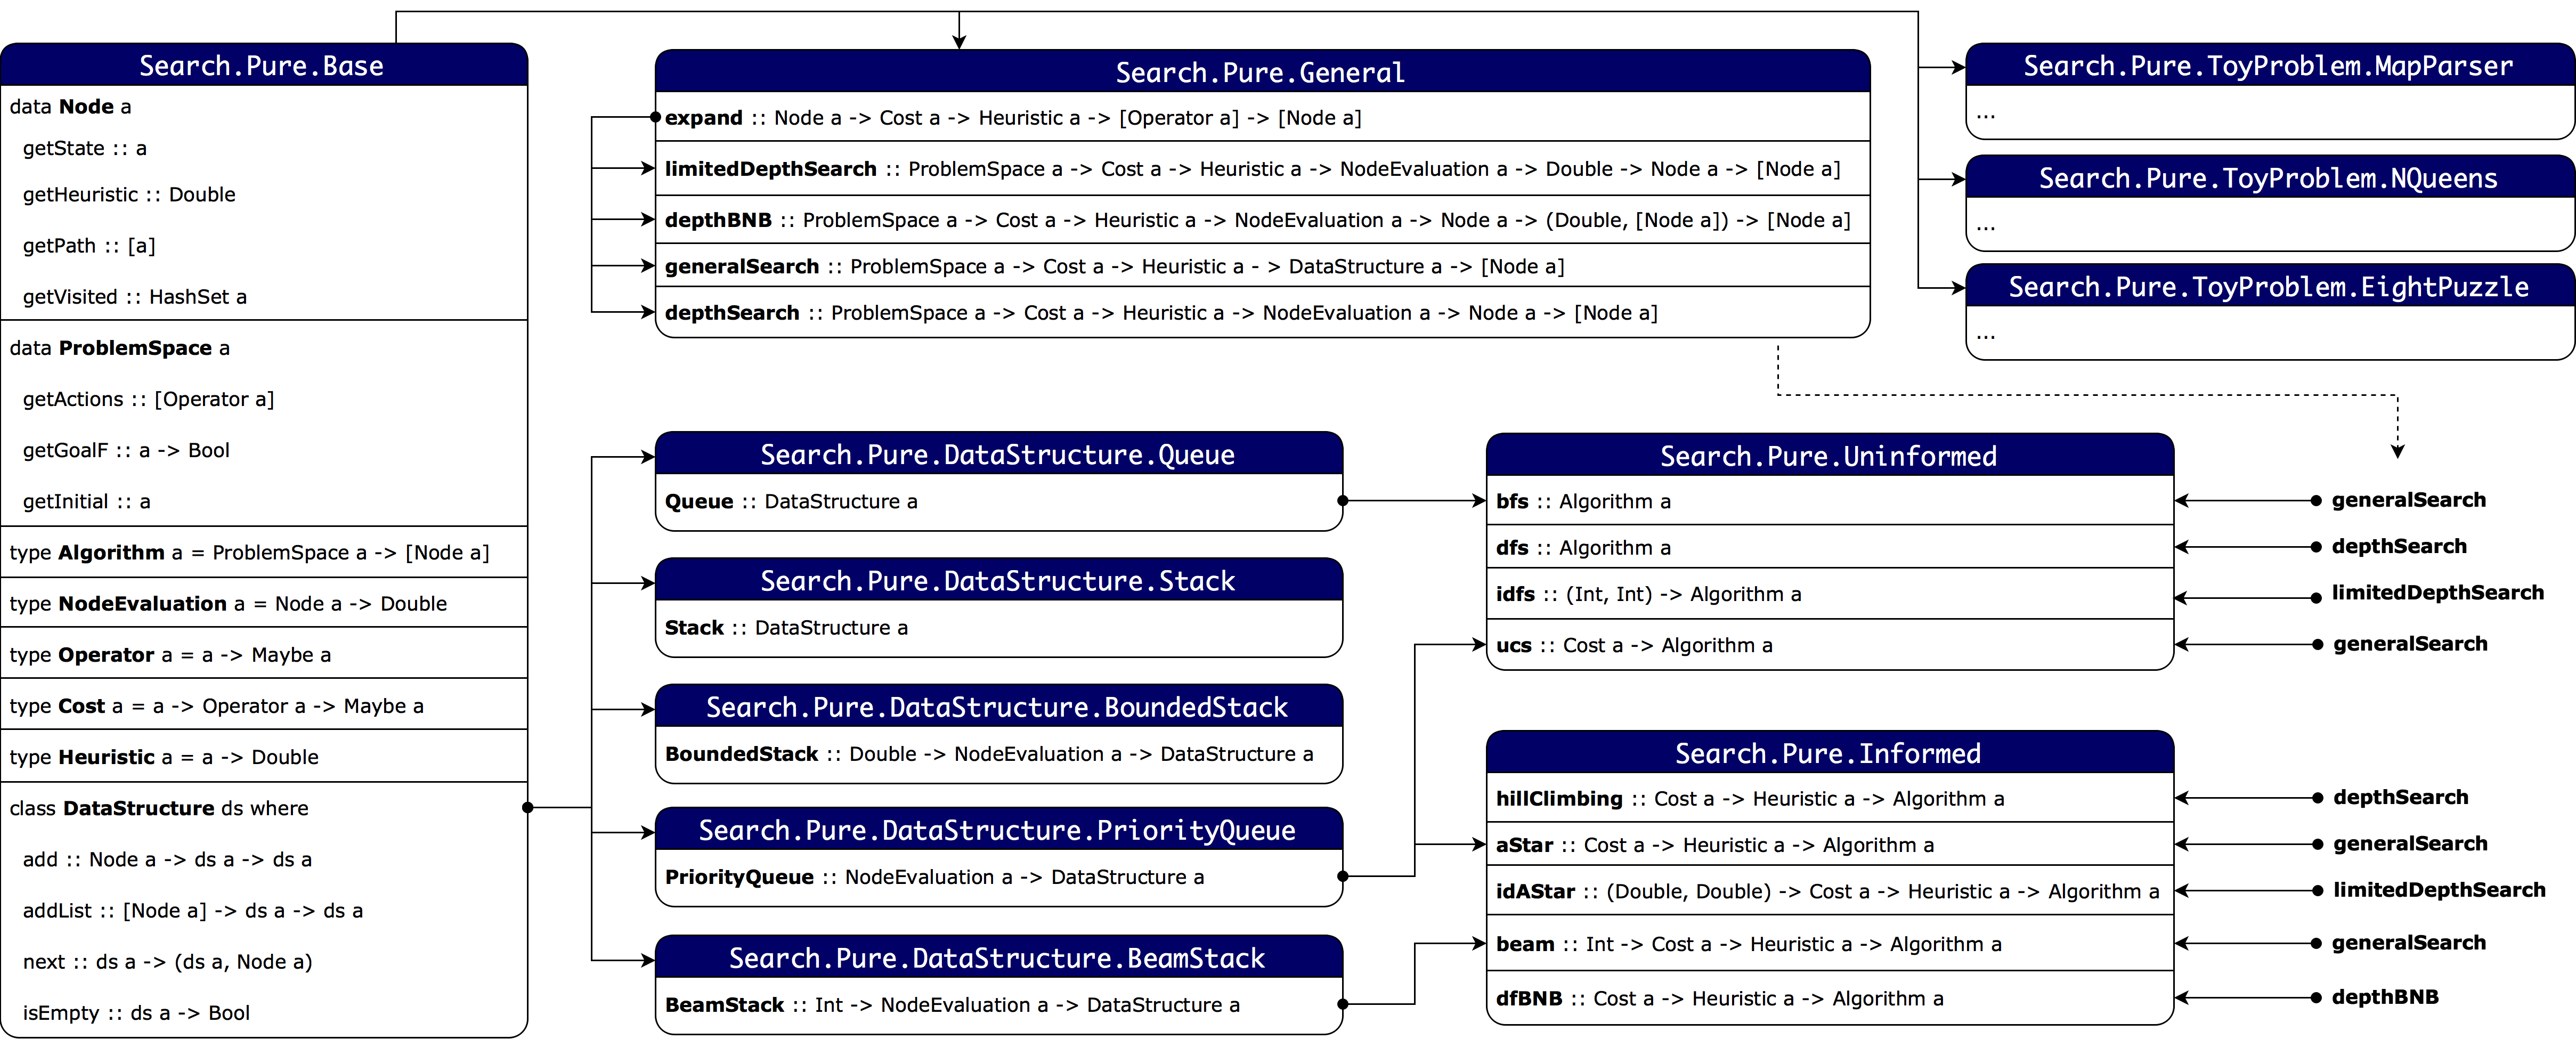
\includegraphics[width=0.9\textwidth]{img/type-graph-pure.png}
  \vspace{1cm}
  \caption{Type signature graph of the \texttt{Search.Pure} library}
  \label{graph-pure}
\end{sidewaysfigure}

\begin{sidewaysfigure}
  \centering
  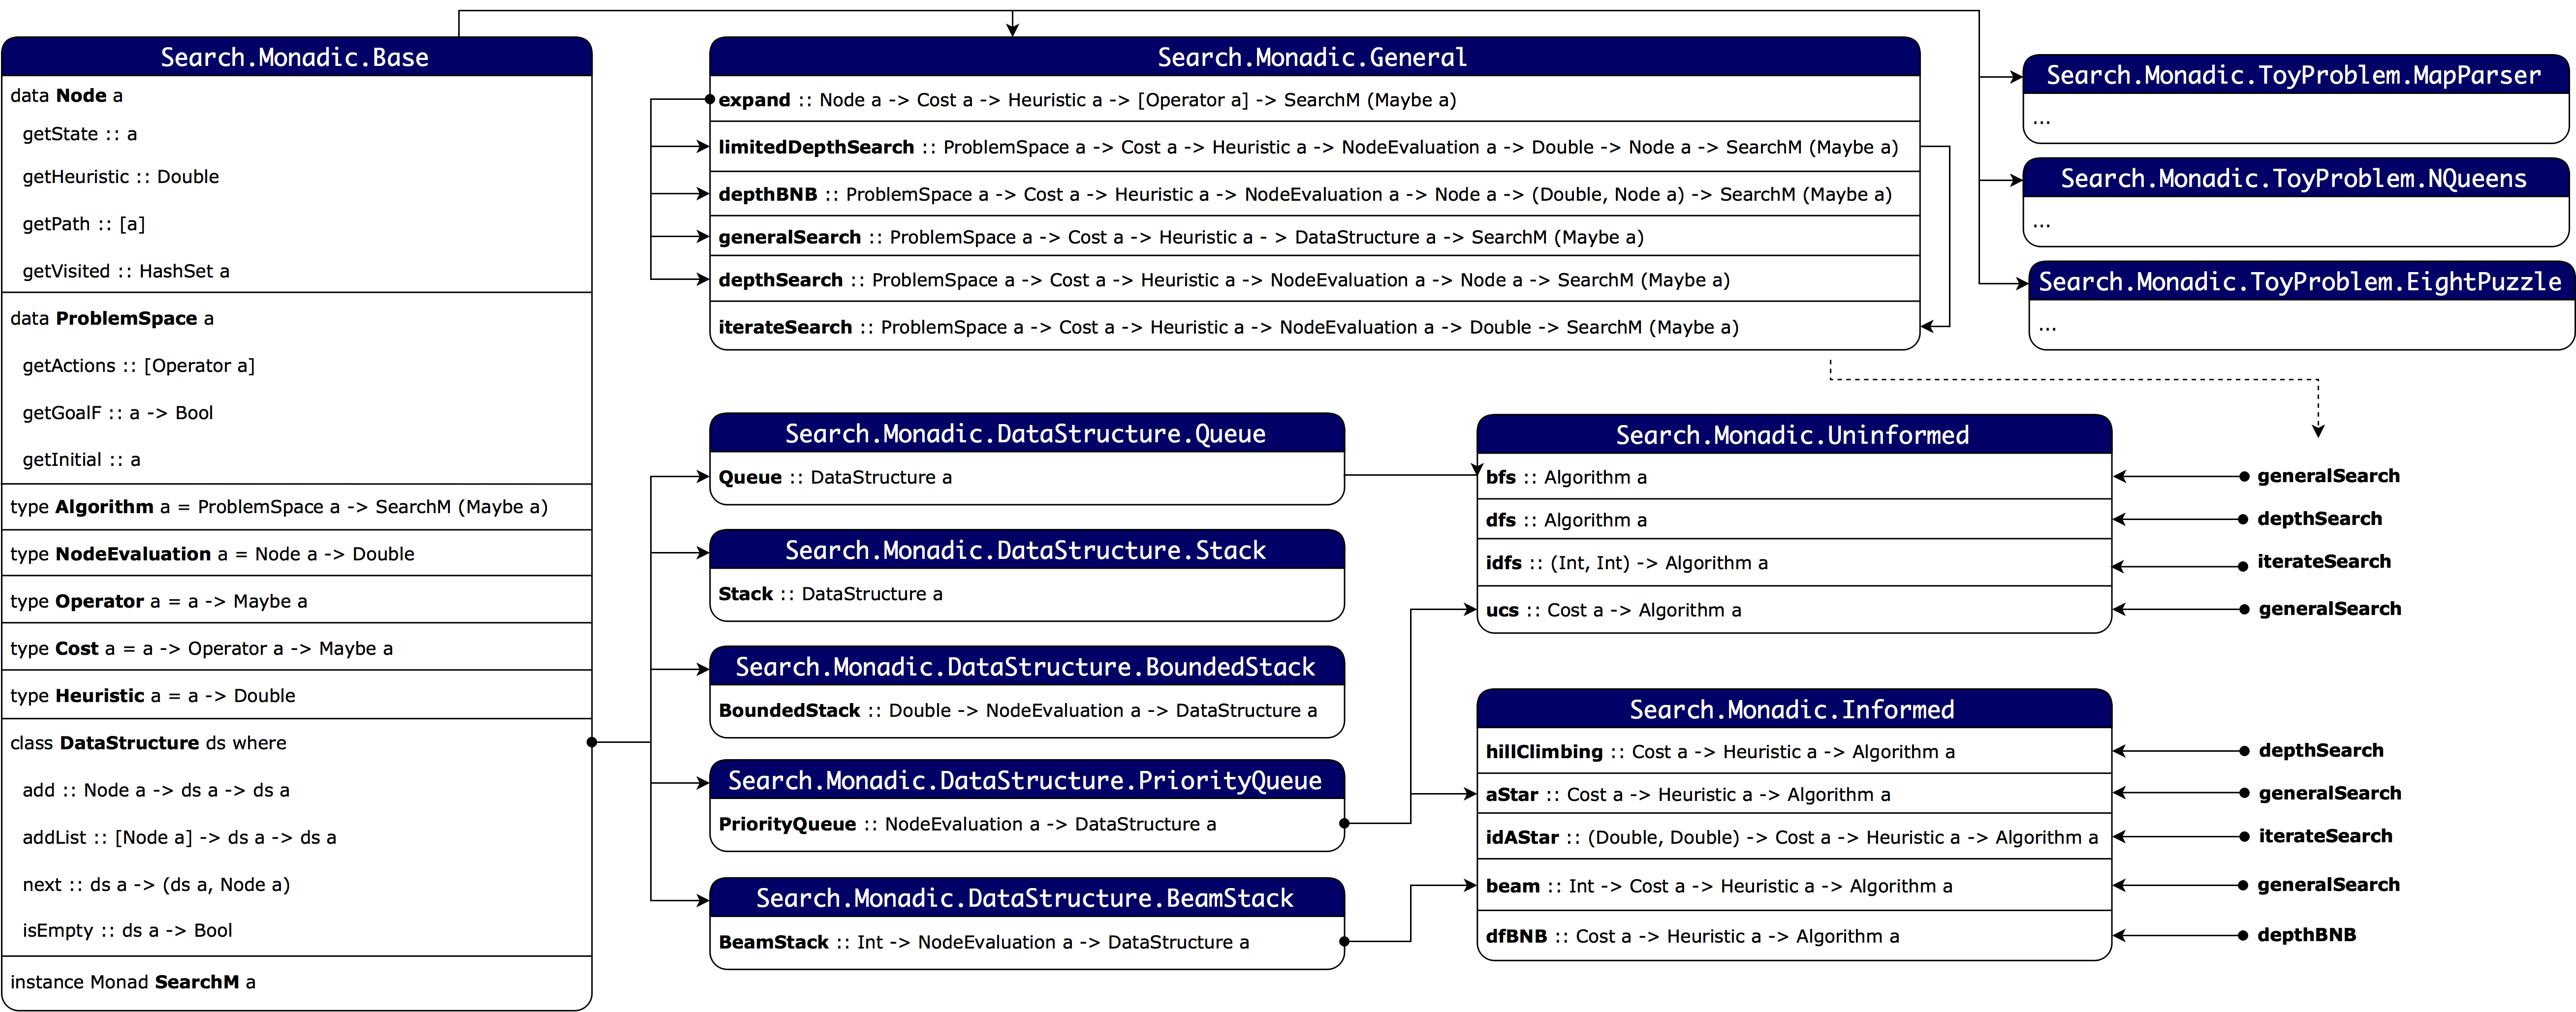
\includegraphics[width=0.9\textwidth]{img/type-graph-monadic.png}
  \vspace{1cm}
  \caption{Type signature graph of the \texttt{Search.Monadic} library}
  \label{graph-monadic}
\end{sidewaysfigure}

These graphs (Figures \ref{graph-pure}, \ref{graph-monadic}) show the basic
control and import flow of the library, and are specially useful for
understanding implementation basics and dependencies among functions. As a
special remark, the specific functions provided by the \texttt{ToyProblem}
modules are omitted (due to lack of interest for the rest of the diagram) as
well as the \texttt{Benchmark} tools, and it is important to notice that every
time the generic type \texttt{a} is mentioned has to follow the constraints
\texttt{Eq a} and \texttt{Hashable a}, since it is the type of the state of the
problem space. Such constraints were dropped from the graph for readability
reasons.\\

We can see how both parts of the library share the same main structure: A
\texttt{Base} module that defines all the main types needed, a \texttt{General}
module that defines the more generalized functions to perform the search, a set
of \texttt{DataStructure} implementations and two modules, \texttt{Uninformed}
and \texttt{Informed} that implement a set of (respectively) uninformed and
heuristic algorithms, using the algorithms and data structures defined in the
former modules. For example, the Breadth-First Search algorithm (\texttt{bfs})
is defined using a \texttt{Queue} data structure and initial conditions of a
\texttt{generalSearch}.\\

Even if both parts of the library seem the same, a closer look reveals that the
monad designed to keep track of the search (\texttt{SearchM}) is returned
instead of a list; a fact that is not visible because it is encapsulated in the
\texttt{Algorithm} type. Also, some noticeable differences like the creation of
new functions to keep better track of search statistics are present in the
\texttt{Monadic} part of the library.\\


\subsection{Implementation}

\subsubsection{General Search}

To perform searches like a Breadth-First search, it is needed to enqueue the
nodes in a structure and check in such structure which one is the next one to
be expanded in the search. This general behavior is mainly modified by the
nature of the data structure used to store the nodes: depending on it, we can
use a queue (for Breadth-First Search), a stack (for a Depth-First Search) or
more complex data structures such as a priority queue (for Uniform-Cost Search
or A* Search, for instance). This general search is indeed described in
\cite{rusell-2003-aima} when first explaining search methods. This algorithm
is the main inspiration for the final implementation of the
\texttt{generalSearch} method.\\

\begin{lstlisting}[style=haskell,
caption=Pure \texttt{generalSearch} implementation, label=pure:general]
generalSearch :: (DataStructure ds, Eq a, Hashable a)
  => ProblemSpace a   -- ^ 'ProblemSpace' to be solved
  -> Cost a           -- ^ 'Cost' function to use
  -> Heuristic a      -- ^ 'Heuristic' function to use
  -> ds a             -- ^ 'DataStructure' that manages the node expansion
  -> [Node a]         -- ^ Returns the list of all final nodes (solutions)

generalSearch problem g h nodes
  | isEmpty nodes                   = []
  | getGoalF problem (getState n)   = n : generalSearch problem g h nodes'
  | otherwise                       = generalSearch problem g h ds'
  where (nodes', n) = next nodes
        expanded = expand n g h (getActions problem)
        ds' = addList expanded nodes'
\end{lstlisting}

We can see in Listing \ref{pure:general} how the implementation is
straightforward: To find all the possible paths to obtain a solution, the
function checks if the node is final and enqueues if to the list of solutions,
or expands it and adds the resulting nodes (if any) to the data structure. This
could keep on going until the data structure is completely empty, but it will
just expand as many nodes as strictly necessary to find the solutions the
function is asked for.\\

This way of relying on the data structure makes a super versatile piece of code
out of this implementation, but also makes it extremely hard to formally prove:
a possible way to do so would be to prove that all the nodes are expanded in a
given order (i.e that a Breadth-First Search expands the nodes in a FIFO way),
but that task depends on the data structure's implementation, so it is not
possible to prove the correctness of this implementation for all possible
entries. To make up for this, we the library includes all unit and integration
tests possible to check correct behavior of it and the default data structures
provided in it.\\

\subsubsection{Linear-Memory Search}

With the \texttt{generalSearch} method we could virtually mimic any possible
algorithm's node expansion order, by adding those functionalities to the data
structure: a stack-like structure will expand nodes in a DFS fashion, adding a
limit of depth will result in an IDFS-like behavior, sorting the nodes in a
priority queue would result in a A* Search. However, stating that all these
behaviors would be a valid implementation of the aforementioned algorithms is a
great underestimation of these designs: there are other aspects to analyze of
an algorithm rather than just the node expansion order
\cite{korf-2014-correct}.\\

A specially problematic aspect for our \texttt{generalSearch} method is the
memory usage: the fact of enqueueing the nodes in the data structure makes it
use an exponential memory depending on the branching factor of the search, and
the fact that the objects in Haskell are immutable only makes this worse. This
is acceptable when performing an A* Search (there is no other way for us to
expand the nodes in order than to sort them in a queue with all the nodes to be
expanded) but trying to use a stack as a data structure to perform a
Depth-First Search will also result in it using exponential memory (all the
nodes get enqueued and passed along the structure). This is not acceptable and
we need to implement a different method for it.\\

Fortunately, implementing this linear-memory method is as easy as relying on
one of Haskell's more natural mechanisms: recursive calls in a tree shape.
However, instead of simple depth-first search, we can take advantage of one of
the most widespread abstractions of the language: \texttt{map}. This function
performs a given function on each of the elements of a list. The main advantage
is that this is one of the abstractions that uses concurrency so may result in
a performance improvement under some certain conditions. In our case, we can
define the method \texttt{depthSearch}, whose pure implementation is defined in
the Listing \ref{pure:depth}.\\

\begin{lstlisting}[style=haskell,
caption=Pure \texttt{depthSearch} implementation, label=pure:depth]
depthSearch :: (Eq a, Hashable a)
  => ProblemSpace a   -- ^ 'ProblemSpace' to be solved
  -> Cost a           -- ^ 'Cost' function to use
  -> Heuristic a      -- ^ 'Heuristic' function to use
  -> NodeEvaluation a -- ^ 'NodeEvaluation' to sort the expanded nodes
  -> Node a           -- ^ Current 'Node' to be expanded
  -> [Node a]         -- ^ Returns the list of all final nodes (solutions)
  
depthSearch problem g h f node
  | getGoalF problem (getState node) = return node
  | otherwise = concatMap (depthSearch problem g h f) sorted
    where sorted = sortBy (\n n' -> compare (f n) (f n')) expanded
          expanded = expand node g h (getActions problem)
\end{lstlisting}

We can see that this implementation includes some interesting mechanics. The
function performs 3 basic tasks: check if a given node contains a final state
inside and leave it, expand non-final nodes and flatten the list. When
flattening the list, the nodes that result in an empty list (that is, that
cannot be expanded) are pruned from the solutions list. By using this, we don't
rely on a sequential implementation and we can take advantage of the
paradigm: this mapping of nodes are actually done concurrently and can increase
the performance compared to a simple recursive call. Also notice that the
function accepts a \texttt{NodeEvaluation} function to sort the nodes. Although
this is not explicitly used in any of the predefined algorithms, can be useful
for an user to sort nodes in order to be expanded.\\

%%% TODO: Diagram explaining work?

However, it is important to note that due to the fact that the each nodes
include in themselves information of their path (the key part to solve the k
path-finding problem) makes the size of the nodes slightly increase as the
search increases. For that reason, the memory is not strictly linear, but it
still provides a huge advantage over the previous method discussed. Since the
memory used is not linear due to the allocation but to the increasing size of
the nodes, this solution will be accepted as good enough for this purpose.\\

This method can be easily modified to perform another type of useful and
widespread linear-memory search: a limited memory search (of any given bound by
the user), that expand nodes if possible or if a given \texttt{NodeEvaluation}
is within the bound given by the user. This function can be read in Listing
\ref{pure:limit}.\\

\begin{lstlisting}[style=haskell,
caption=Pure \texttt{limitedDepthSearch} implementation, label=pure:limit]
limitedDepthSearch :: (Eq a, Hashable a)
  => ProblemSpace a   -- ^ 'ProblemSpace' to be solved
  -> Cost a           -- ^ 'Cost' function to use
  -> Heuristic a      -- ^ 'Heuristic' function to use
  -> NodeEvaluation a -- ^ 'NodeEvaluation' to sort the expanded nodes
  -> Double           -- ^ Limit to be imposed to the 'NodeEvaluation'
  -> Node a           -- ^ Current 'Node' to be expanded
  -> [Node a]         -- ^ Returns the list of all final nodes (solutions)

limitedDepthSearch problem g h f l node
  | getGoalF problem (getState node) = return node
  | otherwise = concatMap (limitedDepthSearch problem g h f l) sorted
    where sorted = sortBy (\n n' -> compare (f n) (f n')) expanded
          expanded = filter ((<l) . f) $ expand node g h (getActions problem)
\end{lstlisting}

With this function, we can implement different search algorithms like
Iterative Depth-First Search or Iterative Deepening A* Search, by performing
a bounded search and increasing the bound over and over.\\

\subsubsection{Branch \& Bound Search}

The last well known general search algorithm that we can provide is a
branch-and-bound fashion search: performing a depth-first search and using the
cost of that solution as the current cost bound. Then, keep on expanding nodes
but making that search be a limited one, by the bound we have found in the
previous solution. Each time a new solution is found, update the bound and keep
on the search until there are no more nodes to expand. This algorithm also uses
linear-space to perform the search, and a pseudocode for it can be found in
\cite{zhang-1995-bnb} along with all necessary explanations.\\

However, this pseudocode is explicitly imperative and seems hard to recreate
using a purely functional approach. A naive approach to this matter would be to
use the previously mentioned algorithms to solve this problem: perform a
\texttt{depthSearch} and store the cost, then perform a
\texttt{limitedDepthSearch} with the current bound and try to found a better
one, and repeat this procedure until no new solution is found. However, this
will not use linear space: instead, it will perform $n$ searches that will,
indeed, use linear-memory each one. This solution is definitely
non-acceptable.\\

The best solution, is to use a fold method, and use such accumulator to hold
both the list of solutions (in a Last In, First Out order) and the current best
cost. Using this fold and recursively calling the function on the nodes, we can
replicate the exact behavior of the algorithm in a purely functional way in a
single search. The code of this function is written in the Listing
\ref{pure:bnb}.\\

\begin{lstlisting}[style=haskell,
caption=Pure \texttt{depthBNB} implementation, label=pure:bnb]
depthBNB :: (Eq a, Hashable a)
  => ProblemSpace a   -- ^ 'ProblemSpace' to be solved
  -> Cost a           -- ^ 'Cost' function to use
  -> Heuristic a      -- ^ 'Heuristic' function to use
  -> NodeEvaluation a -- ^ 'NodeEvaluation' to sort and bound expanded nodes
  -> Node a           -- ^ Current 'Node' to be expanded
  -> (Double, [Node a])    -- ^ The current bound and intermediate solutions
                           -- found (in ascending cost order)
  -> (Double, [Node a])    -- ^ The final bound and all solutions found (in
                           -- ascending cost order)

depthBNB problem g h f n (l, sol) = foldl bnbStep (l, sol) sorted
  where sorted = sortBy (\n n' -> compare (f n) (f n')) expanded
        expanded = expand n g h (getActions problem)

        bnbStep (bound, solutions) n
          | f n >= bound = (bound, solutions)
          | getGoalF problem (getState n) = (f n, n:solutions)
          | otherwise = depthBNB problem g h f n (bound, solutions)
\end{lstlisting}


\subsubsection{Uninformed Algorithms}

Using the previously developed methods, we are able to create a set of
uninformed, purely-functional algorithms ready to use by the users. These
algorithms are just partially-applied general functions which are imposed some
initial conditions to behave as the algorithm is supposed to. Apart from the
convenience that this implies, another main reason to design the search
algorithms this way is because those general search methods are available for
users to build their own search algorithms. Just like these partially-applied
functions result in one algorithm or the other, the users of the framework have
absolute freedom to use them to create their own algorithms.\\

\begin{lstlisting}[style=haskell,
caption=Pure uninformed search algorithms, label=pure:uninf]
-- | 'bfs' runs a Breadth-First Search
bfs :: (Eq a, Hashable a) => Algorithm a
bfs problem = generalSearch problem noCost noHeuristic (startQueue $
                                                        getInitial problem)


-- | 'dfs' runs a Depth-First Search
dfs :: (Eq a, Hashable a) => Algorithm a
dfs problem = depthSearch problem noCost noHeuristic noSorting initial
  where initial = newNode (getInitial problem)


-- | 'idfs' runs an Iterative Deepening Depth-First Search. The first argument,
-- a pair of 'Int's (@step@, @inf@), represent the main parameters of the
-- search: each new iteration the depth test is incremented by adding @step@ as
-- long as the new depth is lower than @inf@.
idfs :: (Eq a, Hashable a) => (Int, Int) -> Algorithm a
idfs (step, inf) p = stepIDFS 0
  where stepIDFS d = if d < inf
          then limitedDepthSearch p noCost noHeuristic depth (fromIntegral d) i
               ++ stepIDFS (d + step)
          else []
        i = newNode $ getInitial p
        depth = fromIntegral . length . getPath


-- | 'ucs' runs an Uniform-Cost Search with a given cost function
ucs :: (Eq a, Hashable a) => Cost a -> Algorithm a
ucs g problem = generalSearch problem g noHeuristic sortedCost
  where sortedCost = startPriorityQueue (getInitial problem) getCost
\end{lstlisting}

In the Listing \ref{pure:uninf} we can see some of the best know brute-force
search algorithms. Breadth-First Search is implemented using a
\texttt{generalSearch} call with a queue data structure (First In, First Out).
On the other hand, the Depth-First Search algorithm uses the simplest
implementation of the \texttt{depthSearch} general method starting in the
initial node of the problem space. Iterative Deepening Depth-First Search is
implemented by performing a \texttt{limitedDepthSearch} over and over,
increasing the depth bound using a given step until that bound is bigger that
some limit given by the user. All these algorithms have been implemented
following the description provided in \cite{rusell-2003-aima}. The last
algorithm in the set is Uniform-Cost Search, which performs a breadth-first,
cost-based search in the problem space. To do so, \texttt{generalSearch} is
used with a priority queue that sorts the nodes in cost ascending order. This
algorithm is usually called Dijkstra's, but this implementation is based on the
description given in \cite{rusell-2003-aima} and due to the nature of the
framework and the language it follows all the criteria exposed in
\cite{felner-2011-dijkstra} to be named Uniform-Cost Search: it works in
implicit graphs (as most all \texttt{ProblemSpace} objects are exactly that),
and Dijkstra's would require to have all nodes input in the $Q$ list.\\


\subsubsection{Informed Algorithms}

In a similar way, we define a set of informed algorithms. The code for these
algorithms can be found in Listing \ref{pure:inf}


\begin{lstlisting}[style=haskell, caption=Pure informed search algorithms,
label=pure:inf]
-- | 'hillClimbing' runs a Hill Climbing Heuristic Search.
hillClimbing :: (Eq a, Hashable a) => Cost a -> Heuristic a -> Algorithm a
hillClimbing g h problem = generalSearch problem g h sortedH
  where sortedH = startPriorityQueue (getInitial problem) getHeuristic


-- | 'aStar' runs an A* Search.
aStar :: (Eq a, Hashable a) => Cost a -> Heuristic a -> Algorithm a
aStar g h problem = generalSearch problem g h sortedAStar
  where sortedAStar  = startPriorityQueue (getInitial problem) aStarF
        aStarF n = getCost n + getHeuristic n


-- | 'idAStar' runs an Iterative-Deepening A* Search.
idAStar :: (Eq a, Hashable a) =>
  (Double, Double) -> Cost a -> Heuristic a -> Algorithm a
idAStar (step, inf) g h p = stepIDAStar 0
  where stepIDAStar l = if l < inf
          then limitedDepthSearch p g h aStarF l initial
               ++ stepIDAStar (l + step)
          else []
        aStarF n = getCost n + getHeuristic n
        initial = newNode (getInitial p)


-- | 'beam' runs a Beam Search of a given beam width.
beam :: (Eq a, Hashable a) =>
  Int -> Cost a -> Heuristic a -> Algorithm a
beam w g h problem = generalSearch problem g h stack
  where stack = startBeamStack (getInitial problem) w getHeuristic


-- | 'dfBNB' performs a Depth-First Branch & Bound Search. Due to the nature of
-- this algorithm, it does not return the list of all solutions in the problem
-- space: Instead, it returns all the solutions that it has found in ascending
-- cost order.
dfBNB :: (Eq a, Hashable a) =>  Cost a -> Heuristic a -> Algorithm a
dfBNB g h problem = snd $ depthBNB problem g h aStarF initial (inf, [])
  where aStarF n = getCost n + getHeuristic n
        initial = (newNode . getInitial) problem
        inf = 1/0
\end{lstlisting}


The first of them is a greedy heuristic search algorithm, better known under
the name of Hill Climbing. This algorithm performs a \texttt{generalSearch}
with a priority queue that sorts the nodes in ascending order of heuristic
value. Arguably, the most popular informed search algorithm, A* Search, is
implemented in a similar way: runs a \texttt{generalSearch} using a priority
queue as well, but that priority queue uses a function $f(n) = g(n) +
h(n)$ to sort the nodes in ascending order, where $g$ is the cost function and
$h$ is the heuristic function. A more lightweight but similar algorithm is
Iterative-Deepening A*, which performs a depth search using the aforementioned
function under a certain bound that increases each new iteration. This searches
take linear time to find the solution, and if IDS performs a search inside a
certain depth, IDA* performs a search inside a certain $f$-spectrum. These
algorithms follow the specifications covered in \cite{rusell-2003-aima}.\\

Another algorithm offered is Beam Search, which uses a data structure called
\texttt{BeamStack} in the library: it only enqueues the best $k$ nodes of a
given expansion, following a \texttt{NodeEvaluation} function. In the previous
case, $k$ is the width of the beam, that is decided by the user. The last
algorithm specified is Depth-First Branch \& Bound, which just uses the
aforementioned \texttt{depthBNB} general method using $f$ as the evaluation
function to perform the Branch \& Bound, as specified in
\cite{zhang-1995-bnb}.\\


\subsubsection{The Search Monad}

These are basically all algorithms provided by the library: a user can import
all these algorithms and model their problem as a \texttt{ProblemSpace}, define
all necessary functions and get the list of solutions. However, if the user is
more interested in an academic or educational point of view, this functions do
not provide some important information: How many nodes are being expanded? How
many nodes where enqueued when we first found a solution?\\

Solving this questions using purely functional reasoning is a real challenge:
the easiest way to do this is using a global variable, outside the scope of the
recursivity, that stores all the necessary statistics. However, since this is
modifying the state of the machine, it is an illegal operation in Haskell. If
we try to use a simple counter we will not obtain always the correct results:
In a depth-first recursion, the counter will only be able to count the expanded
nodes in the solution's path. An accumulator will have a performance cost and
most code should be rewritten to hold it.\\

For those reasons, the solution best solution found for this problem was to use
a monad. A monad is a model that is able to ``bypass'' the explicit data flow
imposed by the pure functional paradigm. This model let us embed a context in a
computation, which is helpful in different situations like error handling,
logging or (like in this specific case) counting operations and execution
traces \cite{wadler-1993-monad}. To do so, the \texttt{SearchM} monad is
included in the library. In this section, its design will be explained as well
as proved correct following the monad laws.\\

\begin{lstlisting}[style=haskell, caption=\texttt{Statistics} implementation,
label=monad:stat]
data Statistics = Statistics
  { nodesExpanded  :: Integer -- ^ Number of nodes expanded through the whole
                              -- search
  , nodesEnqueued  :: Integer -- ^ Number of nodes that have been enqueued
                              -- through the whole search
  , maxQueueLength :: Integer -- ^ Maximum number of nodes that have been
                              -- enqueued at the same time
  } deriving Eq

mergeStats :: Statistics -> Statistics -> Statistics
mergeStats (Statistics exp enq maxL) (Statistics exp' enq' maxL') =
  Statistics (exp + exp') (enq + enq') (max maxL maxL')
\end{lstlisting}

In Listing \ref{monad:stat} we can see the definition of a \texttt{Statistics}
object, which is a record that gathers information about the current search
being performed: the total number of expanded nodes, the total number of nodes
that were added to the data structure, and the maximum size of the data
structure throughout the execution. Also, the method \texttt{mergeStats} is
defined to combine two different statistic logs: sum the expanded and enqueued
nodes and compare the maximum lengths.

\begin{lstlisting}[style=haskell, caption=\texttt{SearchM} implementation,
label=monad:searchm]
data SearchM a = SearchM { getNode  :: a          -- ^ Node with solution
                         , getStats :: Statistics -- ^ Complete search
                                                  -- statistics 
                         }

instance Functor SearchM where
  fmap f (SearchM n stats) = SearchM (f n) stats

instance Applicative SearchM where
  pure n = SearchM n (Statistics 0 0 0)
  SearchM f s <*> SearchM n s' = SearchM (f n) (mergeStats s s')

instance Monad SearchM where
  return = pure
  SearchM n s >>= f = let SearchM n' s' = f n in SearchM n' (mergeStats s s')
\end{lstlisting}

Using the \texttt{Statistics} record, making the monad is a much more
accessible task. In the Listing \ref{monad:searchm} we can see how we define
\texttt{SearchM} as a wrapper for a \texttt{Node} object that contains all the
search statistics. After defining the object, it has to implement all the
necessary classes to be a monad: All monads are also functors (often
endofuctors, since they map a category to themselves) with application and two
natural transformations \cite{street-1972-monads}. For that reason, we have to
define \texttt{fmap} (a generalized version of the \texttt{map} function on
lists) to define it as a functor, and the functions \texttt{pure} (to embed
pure expressions in the functor) and \texttt{<*>} (to sequence computations and
combine their results) to define the application of it.\\

However, by including it as a monad (specially as in a library, as a resource
available to the end user), we need to ensure that it behaves as such. The way
to do it is formally proving that the monad fulfills the monad laws
\cite{wadler-1993-monad}. To prove this, we are going to use the same notation
used in Wadler's work: The bind operator, defined in Haskell as
\texttt{>>=}, will be used in this thesis as $\star$, and lambda clauses will
be defined using the Greek letter ($\lambda$). However, due to a simpler
approach and the increased intuition on the behavior that they provide, the
formulation of the rules will be the ones provided in
\cite{lipovaca-2011-learn}.

\begin{itemize}
\item \textbf{Left identity}: this law states that putting a pure value in
  context and then binding it to a function has to be equivalent to applying
  the function to the variable.

  $$
  unit \  x \star f = f(x) \\
  $$

  Which, in Haskell, is equivalent to the expression \texttt{return x >>= f ==
    f x}, for a variable \texttt{x :: a} and a function \texttt{f :: a -> m b}.
  The formal proof for this law is covered in Listing \ref{monad:leftid}.

\begin{lstlisting}[style = haskell, caption = Left identity formal proof for
\texttt{SearchM}, label = monad:leftid]
return x >>= f == f x
-- { definition of return, where s_id :: Statistics with the identity value }
SearchM x s_id >>= f == f x
-- { definition of >>= }
let SearchM x' s = f x in SearchM x' (mergeStats s_id s) == f x
-- { definition of f }
SearchM x' (mergeStats s_id s) == SearchM x' s
-- { applying identity of s_id }
SearchM x' s == SearchM x' s
-- { equality }
True
\end{lstlisting}

\item \textbf{Right identity}: this law states that binding a monadic value to
  an empty context is no different from the initial monadic value itself.

  $$
  m \star \  \lambda x \rightarrow unit x = m \\
  $$

  This statement can be written in Haskell as
  \texttt{SearchM x s >>= (\symbol{92}x -> return x) = SearchM x s}, for a variable
  \texttt{x :: a}. The formal proof for this law is covered in Listing
  \ref{monad:rightid}.

\begin{lstlisting}[style = haskell, caption = Right identity formal proof for
\texttt{SearchM}, label = monad:rightid]
SearchM x s >>= (\n -> return n) == SearchM x s
-- { definition of return, where s_id :: Statistics with identity value }
SearchM x s >>= (\n -> SearchM n s_id) == SearchM x s
-- { definition of >>= }
SearchM x (mergeStats s_id s) == SearchM x s
-- { applying identity of s_id }
SearchM x s == SearchM x s
-- { equality }
True
\end{lstlisting}

\item \textbf{Associativity}: This law states that the binding of different
  monadic operations is independent of the nesting in which it occurs.

  $$
  m \star f \star g = m \star (\lambda x \rightarrow f(x) \star g)\\
  $$

  For a variable \texttt{x :: a}, and functions \texttt{f :: a -> m b},
  \texttt{g :: a -> m b}, the formal proof for this law is covered in Listing
  \ref{monad:assoc}.

\begin{lstlisting}[style = haskell, caption = Associativity formal proof for
\texttt{SearchM}, label = monad:assoc]
(SearchM x s >>= f) >>= g == SearchM x s >>= (\n -> f n >>= g)
-- { left side - definition of >>= (1); let f x = x'}
SearchM x' (mergeStats s s') >>= g
-- { left side - definition of >>= (2); let g x' = x''}
SearchM x'' (mergeStats (mergeStats s s') s'')
-- { right side - definition of >>= (3); }
SearchM x s >>= (\n -> SearchM ((g . f) n) (mergeStats s_f s_g))
-- { right side - definition of >>= (4); let (f . g) x = x''}
SearchM x'' (mergeStats (mergeStats s' s'') s)
-- { assuming associativity of mergeStats, let result be s_f }
SearchM x'' s_f == SearchM x'' s_f
-- { equality }
True
\end{lstlisting}

  In this proof, the associativity of \texttt{mergeStats} is mentioned as an
  axiom. This can be seen true in Listing \ref{monad:stat} where the
  implementation of this function displays three associative operations: two
  sums and one maximum.\\
  
\end{itemize}


\subsubsection{Adapting the Library to the Search Monad}

Once the monad has been correctly implemented, the library can be replicated
using the monad. However, since,the monad encapsulates context in the
computations to be able to keep track of search statistics. For that reason,
we cannot rely on the lazy evaluation as before: if we ask for the head of the
list of solutions and the statistics, the statistics cover all the computations
to be performed in the whole list, which is an operation that may be endless.
For that reason, it was decided to suppress the idea of returning a list of
solutions in the monadic part of the library: instead, the first solution found
(if any) is returned, as in a traditional search library.\\

If the previous sections have covered the code in the \texttt{Search.Pure} part
of the library, this will instead cover the slight modifications applied to the
code in the \texttt{Search.Monadic} modules to hold the search statistics.
These modifications consists of just modifying the recursive calls inside
do-notation blocks alongside with some logging functions to update the state
embedded inside the monad.\\

These logging functions have a simple mechanism: They create a dummy
\texttt{SearchM} object that will be bind (\texttt{>>=}) to the next object
inside the do-block (do-blocks are indeed just syntactic sugar for a series of
operations bound together \cite{haskell99}). Taking into account that we have
defined the bind operation to replace the object inside the monad and to merge
both object's statistics, this produces the desired outcome.

\newpage

%%% Local Variables:
%%% TeX-master: "tfg"
%%% End:
\section{Testing}

With a functional codebase for the library, it is time to perform all the
necessary tests to ensure the correctness of the code. This is not restricted
to classical unit and integration tests: it is important to perform thorough
analysis of timings to ensure that not only the results are correct, but the
implementation. This analysis is the one that revealed a major leak in the
library, and all the work done to try to fix it is gathered in this section.\\

\subsection{Search Domains Analysis}

After performing the unit testing, the library still has to be proven reliable
and fast in different search domains. To do so, we will use these domains:

\begin{itemize}
\item \textbf{N-Queens}: This problem consists in placing $n$ queens in a $n
  \times n$ chess board so that no two queens are in the same row, column or
  diagonal: that is, placing all the queens without two queens threatening each
  other. This problem is provided in the library under the module
  \texttt{Search.[...].ToyProblem.NQueens}, and this is the implementation that will
  be used to test the performance.
\item \textbf{8-Puzzle}: This problem uses a $3 \times 3$ board that contains 8
  numerated tiles and a blank space. The tiles can be slide around the board if
  they are next to the blank space, and the purpose of the puzzle is to end up
  with a sorted board. This problem is provided in the library under the module
  \texttt{Search.[...].ToyProblem.EightPuzzle}.
\item \textbf{Moving AI Maps}: This problem depends receives a map and two
  coordinates, and the agent generated tries to find a path that goes from one
  point to the other. Depending on the algorithm, this path will be the easier
  to find or the shortest. The map file is expected to be in the format
  provided by \cite{movingai-benchmarks}. This is the most demanding problem of
  all to be tested, as well as the most versatile. A parser for this kind of
  maps is included in \texttt{Search.[...].ToyProblem.MapParser}.
\end{itemize}

In each problem, a different capability of the library is tested, and it will
be explained in depth in each of the domains subsections. To perform these
tests, the included tools with the library will be used to perform all
measurements.\\

\subsubsection{Results and Performance in N-Queens}

\begin{figure}[!htbp]
  \centering
  \begin{tikzpicture}
    \begin{axis}[
      ybar,
      axis lines*=left,
      every axis plot post/.style={/pgf/number format/fixed},
      enlargelimits=0.15,
      x = 2.3cm,
      bar width = 0.8cm,
      legend style={at={(0.5,-0.15)},
        anchor=north,legend columns=-1},
      ylabel={Time (ms)},
      symbolic x coords={BFS,DFS,IDFS(1),IDFS(5),UCS},
      xtick=data,
      nodes near coords,
      nodes near coords align={vertical},
      ]
      \pgfplotsset{cycle list name=list}
      \addplot coordinates {
        (BFS,125.5)
        (DFS,6.806)
        (IDFS(1),352.0)
        (IDFS(5),38.0)
        (UCS,137.1)
      };
      % \legend{}
    \end{axis}
  \end{tikzpicture}
  \caption{Time to find a solution in 8-Queens}
  \label{nq:time}
\end{figure}


\begin{figure}[!htbp]
  \centering
  \begin{tikzpicture}
    \begin{axis}[
      compat=newest,
      axis lines*=left,
      every axis plot post/.style={/pgf/number format/fixed},
      ybar,
      enlargelimits=0.15,
      x = 2.3cm,
      bar width = 0.8cm,
      legend style={at={(0.5,-0.15)},
        anchor=north,legend columns=-1},
      ylabel={Nodes expanded},
      symbolic x coords={BFS,DFS,IDFS(1),IDFS(5),UCS},
      xtick=data,
      nodes near coords,
      nodes near coords align={vertical},
      ]
      \pgfplotsset{cycle list name=list}
      \addplot coordinates {
        (BFS,1966)
        (DFS,114)
        (IDFS(1),5623)
        (IDFS(5),650)
        (UCS,1966)
      };
      % \legend{}
    \end{axis}
  \end{tikzpicture}
  \caption{Nodes expanded to find a solution in 8-Queens}
  \label{nq:nodes}
\end{figure}


\begin{figure}[!htbp]
  \centering
  \begin{tikzpicture}
    \begin{axis}[
      compat=newest,
      ybar,
      axis lines*=left,
      every axis plot post/.style={/pgf/number format/fixed},
      enlargelimits=0.15,
      x = 2.3cm,
      bar width = 0.8cm,
      legend style={at={(0.5,-0.15)},
        anchor=north,legend columns=-1},
      ylabel={Total Memory Allocated (KB)},
      symbolic x coords={BFS,DFS,IDFS(1),IDFS(5),UCS},
      xtick=data,
      nodes near coords,
      nodes near coords align={vertical},
      ]
      \pgfplotsset{cycle list name=list}
      \addplot coordinates {
        (BFS,72840)
        (DFS,6066)
        (IDFS(1),152132)
        (IDFS(5),20164)
        (UCS,68501)
      };
      % \legend{}
    \end{axis}
  \end{tikzpicture}
  \caption{Total memory allocated to find a solution in 8-Queens}
  \label{nq:memory}
\end{figure}

The implementation for the N-Queens problem included with the library uses as
operators the fact of adding a queen to a new column in all possible positions.
That way, the approach followed to solve this problem is a brute-force
approach, which is ideal to study all the uninformed algorithms. On the other
hand, there is no heuristic available for this approach, so the informed set of
algorithms cannot be tested in this domain. For the same reason, no correctness
of the solution has to be considered: if the solution is found is because it is
valid. That makes the evaluation simpler to understand for this case.\\

We can see a clear correlation between the time taken find a solution (Figure
\ref{nq:time}) and the nodes expanded in the process (Figure \ref{nq:nodes}).
The results are not surprising: We can see how Breadth-First Search takes some
a fair amount of time to find the solution, but the algorithm has to traverse
completely some depths of the tree that cannot contain solutions, which makes
a handicap for this algorithm. It is also noticeable that the best algorithm
for this brute-force search is Depth-First Search, which is the fastest
algorithm. Also an important insight is the fact that Iterative-Deepening
Depth-First Search is quite sensitive to the parameters given: appropriate step
parameters can save up to an order of magnitude in the nodes expanded.
Uniform-Cost Search also behaves as a Breadth-First Search, since there is no
variable cost function for this concrete example. In the Figure
\ref{nq:memory}, we can see the total amount of memory allocated during the
process; not the total memory used by it (memory is claimed back at some
moments when it stops being used). The correlation between nodes and memory
allocated is clear as well.\\

It is also interesting to check the results of the benchmarks for counting all
the solutions in the search domain. This test is specially interesting with
Breadth-First Search and Depth-First Search: both of them should find the same
number of solutions (92 for 8-Queens) and expand all nodes in the search space.
The differences between timing will show if there is an intrinsic difference in
the language in both approaches:\\

\begin{lstlisting}
<lambda> benchmark $ withAllNQueens [("bfs", bfs), ("dfs", dfs)]
benchmarking nQueens/bfs
time                 116.3 ms   (113.9 ms .. 119.5 ms)
                     0.999 R²   (0.998 R² .. 1.000 R²)
mean                 116.6 ms   (115.9 ms .. 117.6 ms)
std dev              1.247 ms   (772.9 µs .. 1.917 ms)
variance introduced by outliers: 11% (moderately inflated)

benchmarking nQueens/dfs
time                 111.9 ms   (110.4 ms .. 114.1 ms)
                     1.000 R²   (0.999 R² .. 1.000 R²)
mean                 113.3 ms   (112.6 ms .. 114.1 ms)
std dev              1.149 ms   (803.0 µs .. 1.613 ms)
variance introduced by outliers: 11% (moderately inflated)
\end{lstlisting}

The results show that both algorithms find the set of solutions using almost
the same amount of time: Depth-First Search is just 2.5\% faster than
Breadth-First, probably because of the time saved in allocating memory for the
data structure, which is substituted by stack calls. These are good news: In
this search domain, when finding all possible solutions, using linear search
memory or a general search with a data structure have no visible time overhead
from one another.\\

\subsubsection{Results and Performance in 8-Puzzle}

In the implementation available in the library for 8-Puzzle, the operators
consists of moving the blank space in the board. It is just a simpler way to
express, the problem, and it works the same way as moving the tiles to the
blank space. Thus, the complexity in this puzzle is much higher than in
N-Queens, where a brute force search was proven to be quite efficient.
Fortunately, there is an advantage compared to the previous problem: we can
design heuristic functions to help us with it, and use the informed set of
algorithms at hand. Included in the module there is a basic heuristic for this
problem: the hamming heuristic, which counts how many numbers are not in the
correct position.\\

It is important to notice that the initial position of the board to perform
these tests is the one provided in the library for benchmarking puzzles. This
initial position has an optimal solution of 17 steps before being solved. We
will then specify the correctness of the solutions found by the algorithm, but
first we can check the times taken by each of them.\\

\begin{figure}[!htbp]
  \centering
  \begin{tikzpicture}
    \begin{axis}[
      compat=newest,
      every axis plot post/.style={/pgf/number format/fixed},
      ybar=5pt,
      enlargelimits=0.28,
      x = 1.5cm,
      ymax = 1600,
      bar width = 0.8cm,
      legend style={at={(0.5,-0.15)},
        anchor=north,legend columns=-1},
      ylabel={Time (ms)},
      symbolic x coords={BFS,DFS,IDFS,HC,A*,IDA*,BNB},
      xtick=data,
      restrict y to domain*=0:2300,
      visualization depends on=rawy\as\rawy,
      after end axis/.code={ % Draw line indicating break
        \draw [ultra thick, white, decoration={snake, amplitude=1pt},
        decorate] (rel axis cs:0,1.05) -- (rel axis cs:1,1.05);
        },
    nodes near coords={%
            \pgfmathprintnumber{\rawy}% Print unclipped values
          },
      axis lines*=left,
      clip=false
      ]
      \pgfplotsset{cycle list name=list}
      \addplot coordinates {
        (BFS,1327)
        (DFS,59.53)
        (IDFS,1464)
        (HC,701.2)
        (A*,234.6)
        (IDA*,113.4)
        (BNB,44396)
      };
      % \legend{}
    \end{axis}
  \end{tikzpicture}
  \caption{Time to find a solution in 8-Puzzle}
  \label{8p:time}
\end{figure}

In the Figure \ref{8p:time} we can see the times taken to solve this puzzle.
The uninformed algorithms perform as expected: Breadth-First Search takes a
fair amount of time but ensures that the solution is optimal, while Depth-First
Search takes a short time to find the first solution available. Iterative
Deepening Depth-First Search performs worse than BFS without any warranties,
but it can be tuned later with better parameters to improve the times
obtained.\\

On the other hand, we see for the first time results on the informed
algorithms. Hill Climbing takes almost half the time taken by BFS, but it is
important to notice that it is simply following greedily the heuristic
function, so it will not always return the optimal solution. On the other hand,
A* uses both the cost function and the heuristic function, ensuring that the
obtained solution is the optimal. Also, A* performs really good: it's around
seven times faster than BFS, and the results are indeed the same.
Iterative-Deepening A*, on the other hand, uses linear memory, but if the
parameters are not correct the solution found it's not going to be optimal. We
can see that IDA* is twice as fast as A*.\\

However, we can see that Depth-First Branch and Bound is much slower than the
rest of the available algorithms. Although it produces the optimal solution, it
is several orders of magnitude slower, which makes it not acceptable. The
reason for this is that the rest of the algorithms are obtaining one single
solution: The first solution that they are able to find. On the other hand,
Branch and Bound uses the first solution as a bound, and then keeps on searching
until the solution space is completely exhausted. That makes BNB not being able
to take advantage of Haskell's laziness as the other algorithms, and resulting
in a terrible performance in this search domain, since the search space is hard
to completely explore. That makes Depth-First Branch and Bound a bad choice for
this problem.\\

\begin{figure}[!htbp]
  \centering
  \begin{tikzpicture}
    \begin{axis}[
      compat=newest,
      every axis plot post/.style={/pgf/number format/fixed},
      ybar=5pt,
      enlargelimits=0.21,
      x = 1.5cm,
      bar width = 0.7cm,
      axis lines*=left,
      legend style={at={(0.5,-0.15)},
        anchor=north,legend columns=-1},
      ylabel={Steps},
      symbolic x coords={BFS,DFS,IDFS,HC,A*,IDA*,BNB},
      xtick=data,
      nodes near coords,
      nodes near coords align={vertical},
      ]
      \pgfplotsset{cycle list name=list}
      \addplot coordinates {
        (BFS,17)
        (DFS,1053)
        (IDFS,18)
        (HC,88)
        (A*,17)
        (IDA*,17)
        (BNB,17)
      };
      % \legend{}
    \end{axis}
  \end{tikzpicture}
  \caption{Steps to solve the problem in each solution found}
  \label{8p:steps}
\end{figure}

In Figure \ref{8p:steps} we can see the quality of each algorithm's answer to
the problem. The shorter the solution found, the better the solution is, and
the optimal solution for the instance being tested is 17 steps. We can see how,
in this example, the algorithms that are able to find that solution are BFS,
A*, IDA*, and BNB; with IDFS is really close to it. Unsurprisingly, the greedy
algorithms (DFS and Hill Climbing) do not find optimal solutions, but their
time/memory performance is overall better.\\

\subsubsection{Results and Performance in Moving AI Maps}

The Moving AI maps are the most complex and demanding test of all. These maps
are formed by a $512 \times 512$ grid that contain walls and different sets of
terrains. The first test, to test the timing and different behaviors of the
algorithms, will be performed in a maze with corridors of width 1. That means
that the problems only have to check paths at different intersections, making
the branching factor smaller. There is a single solution, with a length of 5172
nodes until the goal state. The results to this test are:\\

\begin{figure}[!htbp]
  \centering
  \begin{tikzpicture}
    \begin{axis}[
      compat=newest,
      every axis plot post/.style={/pgf/number format/fixed},
      ybar=5pt,
      enlargelimits=0.21,
      x = 1.5cm,
      bar width = 0.7cm,
      legend style={at={(0.5,-0.15)},
        anchor=north,legend columns=-1},
      ylabel={Time (ms)},
      symbolic x coords={BFS,DFS,IDFS,HC,A*,IDA*,BNB},
      xtick=data,
      axis lines*=left,
      nodes near coords,
      nodes near coords align={vertical},
      ]
      \pgfplotsset{cycle list name=list}
      \addplot coordinates {
        (BFS,0.559)
        (DFS,0.256)
        (IDFS,10.126)
        (HC,7.453)
        (A*,20.014)
        (IDA*,0.684)
        (BNB,0.392)
      };
      % \legend{}
    \end{axis}
  \end{tikzpicture}
  \caption{Time to find a solution in the $512 \times 512$ maze}
  \label{mp:time}
\end{figure}

There are three things that catch our eye in these results: the great
discordance between the two iterative-deepening methods (applied with similar
parameters to the problem), the great performance of Depth-First Branch and
Bound and the terrible performance of A*.\\

The first one can be explained in function of the maze itself. It is (in this
case) much more effective to follow greedily the heuristic function rather than
expanding the search tree depth-first. This is translated in IDA* needing much
less iterations than IDFS. However, this contradicts the fact that BFS is much
more performant than Hill Climbing. We will come back to this detail.\\

Second, Depth-First Branch and Bound has proven to be a good option to solve
this concrete problem, being only slower than DFS. This also ensures that the
problem the algorithm suffered in the previous section are not intrinsic to the
implementation, but to the nature of the problem and the algorithm.\\

But the really surprising measure is A*: how can the algorithm that was the
better performing until now, suddenly performs much more slower than the rest
of algorithms. How is it possible than an A* search is an order of magnitude
slower than its BFS counterpart? After all the previous testing on the code, it
is possible to state that concrete conditions are resulting in slow conditions
for A*. Incidentally, there is also a noticeable slower performance for Hill
Climbing, specially after noticing that it should be favored by the heuristic
function in this scenario. This two algorithms share something in common: both
of them are implemented using a priority queue
(\texttt{Search.[...].DataStructure.PriorityQueue}). Knowing this, our next
step is to try to figure out what is causing this degradation for the priority
queue or if it is something else. This will be studied more comprehensively in
the following profiling section.\\

Furthermore, if the Moving AI Benchmarks can find the real Achilles' heel of
the library: due to its purpose of finding the best $k$ solutions for a given
problem, when we try to run demanding pathfinding problems in corridors of
width $>1$, the algorithms revisits the same nodes as long as its own path does
not contain it. In problems based in implicit graphs, it usually means an
admissible redundancy; in problems based in maps this implies that the number
of paths being tracked is higher and in algorithms like Breadth-First Search
(that expands the nodes with lower depth first) the algorithm struggles to
advance to the final solution \cite{dechter-2012-search}. For that reason, it
is recommended to use a traditional approach for different maps and mazes.\\

\subsection{Unit and Integration Testing}

Thanks to the Cabal packaging tool, it is easy to include a test suite in the
library, that can be run automatically. The chosen way to test the functions of
the library was to create a \texttt{Test} folder, in which replicate the
structure of the library modules. In each of this new modules there should be
all the tests for the functions included in them. Since the design of the
library functions are incremental, these small specifications can be both unit
tests (for instance, to check if \texttt{Search.DataStructure.Queue} correctly
adds a node) or integration tests (if a queue and a general search can be
combined correctly to work as a Breadth-First Search). To perform the latter
tests, we will use small examples of each of the search domains that have been
included in the library as toy problems, to test the correctness of the results
returned.\\

To perform this task, the easiest way is to use the \texttt{hspec} package,
that offers all the necessary functions to perform the testing of the modules,
plus a function to discover and run all necessary \texttt{Spec} files when
asking the library to be tested. That way, we can just create new test modules
and they will be automatically discovered. To run the tests it is only
necessary to build the library along with the tests (\texttt{cabal build
  --enable-tests}) and then run \texttt{cabal test}. This convenient access to
the tests is the cornerstone for the Continuous Integration of the library,
that will be specified later on the document.\\

Running this command in the version for this thesis (\texttt{0.2.0.0}) runs a
total of 156 different examples (both unit and integration tests) in
$\sim 2.6581$ seconds with 0 failures. The output presents the name of each of
the modules being tested, along with a description of each of the tests and a
mark in case there was a failure in such example. The complete set of tests can
be found in the path \texttt{src/Test/} of the library code.\\

\subsection{Profiling}

As seen in previous sections, the library has an overall good performance, but
under certain conditions the it becomes drastically slower. However, it is hard
to say what is exactly happening: due to the side-effects isolation, there is
no easy way to use print-debugging or to time different functions of the code
to see what is exactly going on. At this level of abstraction, what the
computer is doing in the bad performances is, indeed, completely hidden from
us.\\

However, the language provides certain tools to profile code if it is indeed
necessary to spot a problem. The main tool for profiling is using the
\texttt{+RTS} interface, that will be detailed next. After explaining the
process of creating a working environment to profile the project, we will
undergo several experiments to find the hot spots in the project and follow a
procedure to fix it.\\

\subsubsection{Creating the \texttt{profiling} executable}

To effectively profile code in Haskell, it is needed to make use of an
interface to the Runtime System (RTS). This system, which is not usually
intended to be directly queued, is the one in charge of a lot of Haskell's nuts
and bolts: RTS includes a storage manager, a scheduler and a profiler, among
other necessary runtime services that work as a middle system between the user
code and the compiled Haskell code \cite{ghc}.\\

To effectively profile the code, it is necessary to use both compilation and
runtime flags. This is usually easy to manage with single files, but a project
like this can become really hard to compile with a simple \texttt{ghc} command
outside of a packaging tool like Cabal or Stack. Plus, the library needs to
install the profile version of the dependencies, so simply compiling by hand
may not be enough to successfully profile the code.\\

The best solution available for a project this size is to create a Cabal
executable that will gather all the options, and enables for an easy access to
the profiling of the library. To create this executable, we need to add the
Listing \ref{prof-cabal} to the file \texttt{agis.cabal} in the root of the
project.\\

\begin{lstlisting}[style=haskell, label=prof-cabal, caption=
Setup for the \texttt{profiling} executable in the Cabal file]
-- Library profiling executable
executable profiling

  hs-source-dirs:      src/Search/Pure
           
  main-is:             Profiling.hs
  
  ghc-options:         -O2
                       -threaded
                       "-with-rtsopts=-N -p -s -h -i0.1"

  build-depends:       [...]

  default-language:    Haskell2010
\end{lstlisting}

This configuration creates a new executable called \texttt{profiling}, that
will call the file \texttt{Profiling.hs} in the directory
\texttt{search/Search/Pure}. This file will simply contain a main method
calling the code to be tested, which will be the main method for the Moving AI
maps. For this executable to created, we pass several options to the compiler:
to be compiled with level 2 optimizations (\texttt{-O2}) and using the
concurrent abstractions (\texttt{-threaded}), as well as to include all the
necessary runtime options (\texttt{-with-rtsopts}):

\begin{itemize}
\item \texttt{-N} sets the number of available processors to the number of
  processors of the system.
\item \texttt{-p} generates the profiling report.
\item \texttt{-s} includes garbage collection in the report.
\item \texttt{-h} includes memory usage in the report.
\item \texttt{-i} sets the profiler frequency to 0.1 seconds.  
\end{itemize}

Running \texttt{cabal build} will compile the project (and install all the
necessary profiling version of the dependencies) and generate the executable.
To run it, it is only necessary to run \texttt{cabal run profiling}. This
shortcut is much more robust and simple than to input the compiler flags every
time. Once run, it outputs a brief description of the profiling in the memory
and generates a comprehensive report (a \texttt{.prof} file) where the runtime
statistics are detailed. Now that the environment is set, we can proceed to
profile the code searching for the hot spots in the library.\\


\subsubsection{Finding the hot spots of the library}

As it could be seen when testing the library with the Moving AI maps, there is
a problem related to the priority queue implementation of the library. There
are several possible causes for this, and to better find out what the problem
may be, we need to use the aforementioned profiler. An open map will be used to
profile the code, and try to see where the hot spots of time and memory
allocation are.\\

To do so, it is necessary to use GHC's cost centres: A special annotation that
precedes a statement and lets the compiler know that it is a point of interest.
All the cost centres will then be collected in the \texttt{.prof} report, that
contains a comprehensive analysis of how the code is behaving \cite{ghc}. A
cost centre is included in the code using \texttt{\{-\# SCC "name" \#-\}
  <expression>}, and it will track and include in the report the total time and
memory usage of the expression under the row \texttt{name}.\\

Running the example with some functions being tracked results in the following
report:\\

\begin{lstlisting}
	Sun Jul 23 15:28 2017 Time and Allocation Profiling Report  (Final)

	   profiling +RTS -N -p -s -h -i0.1 -RTS

	total time  =        3.48 secs   (3479 ticks @ 1000 us, 1 processor)
	total alloc = 2,730,181,144 bytes  (excludes profiling overheads)

COST CENTRE   MODULE                           %time %alloc

union         Data.Heap.Internal                47.1   30.3
getCell       Search.Pure.ToyProblem.MapParser   8.8    5.0
move          Search.Pure.ToyProblem.MapParser   6.7    9.5
visited       Search.Pure.General                6.6    0.3
generalSearch Search.Pure.General                5.7   13.0
fromList      Data.Heap                          4.7   10.8
expand        Search.Pure.General                4.7    6.4
size          Data.Heap.Internal                 3.3    7.7
rank          Data.Heap.Internal                 2.6    7.4
expand        Search.Pure.General                1.3    4.1
cost          Search.Pure.General                1.1    0.9
heuristic     Search.Pure.General                1.1    0.4
hash          Data.HashMap.Base                  1.1    0.0
readWMap      Search.Pure.ToyProblem.MapParser   0.3    1.6
\end{lstlisting}

We can see how more than half of the time is being consumed in the library
calls of \texttt{Data.Heap}. This is provided by the package \texttt{heap},
which allows import a \texttt{MinHeap}, the basic data structure on top of
which is built our own implementation of a purely functional priority queue,
as described in \cite{okasaki-1999-purely}. We can see that the library is
generating a time overhead that is not acceptable, but apart from the report,
there is a key statement in the RTS briefing that appears in the prompt:\\

\begin{lstlisting}
> cabal run profiling
   4,668,660,936 bytes allocated in the heap
   4,684,133,240 bytes copied during GC
     183,250,168 bytes maximum residency (44 sample(s))
       1,394,480 bytes maximum slop
             371 MB total memory in use (0 MB lost due to fragmentation)

                                     Tot time (elapsed)  Avg pause  Max pause
  Gen  0      8972 colls,     0 par    0.998s   1.024s     0.0001s    0.0031s
  Gen  1        44 colls,     0 par    5.425s   5.637s     0.1281s    0.2877s

  TASKS: 4 (1 bound, 3 peak workers (3 total), using -N1)

  SPARKS: 0 (0 converted, 0 overflowed, 0 dud, 0 GC'd, 0 fizzled)

  INIT    time    0.001s  (  0.013s elapsed)
  MUT     time    3.390s  (  4.697s elapsed)
  GC      time    5.127s  (  5.354s elapsed)
  RP      time    0.000s  (  0.000s elapsed)
  PROF    time    1.296s  (  1.306s elapsed)
  EXIT    time    0.003s  (  0.051s elapsed)
  Total   time    9.818s  ( 10.116s elapsed)

  Alloc rate    1,377,217,805 bytes per MUT second

  Productivity  34.6% of total user, 34.0% of total elapsed
\end{lstlisting}

In there, we can see how the \texttt{MUT} (actual computations that are being
issued) take 3.390s; but \texttt{GC} (the garbage collector, that claims back
the memory not being used) is generating more than 5 seconds in pauses.
Overall, the productivity of the code (the fraction of the execution that is
invested in the actual computations) is 34.6\%: only one out of each three
seconds of execution. The main responsible for this situation is the garbage
collector, and there are two main possibilities for this: the library code is
being misused and the compiler is not able to execute the proper optimizations
on it, or the garbage collection settings are affecting the performance.\\

\subsubsection{Tuning the garbage collection}

After running the profiling experiments in the code, we have found that
problems with a fast growing queue generate a problematic space overhead, that
is translated to big garbage collection pauses that make execution slow. The
cost centers reveal that the space allocation happen most of all in the
\texttt{DataStructure} methods for adding nodes, so let us keep researching how
to fix this issue. To generate a lot of nodes in the open list, we will use a
bad heuristic in the problem \texttt{MapParser}, to get a solution with these
statistics (obtained with the \texttt{Search.Monadic} library):

\begin{itemize}
 \item Number of expanded nodes: 378790
 \item Number of enqueued nodes: 734887
 \item Maximum length of the queue: 356099
\end{itemize}

Just to obtain a plan length of 19. This big size for the open list will
trigger the garbage collection problem and let us study it better. The mean
execution time for this problem in the original implementation is 11.573
seconds; which may seen acceptable but increases rapidly with the plan length
(a new node can add 8-10 seconds to this execution time).\\

Now, to experience the impact of the garbage collector settings we will use a
tool called \texttt{ghc-gc-tune} \cite{ghc-gc-tune}. This tool will allow us to
brute force the garbage collector options and get a general insight of the
behavior of the program under different settings. This will let us see if the
problem is originated by the garbage collector being too intrusive or if there
is a reason intrinsic to the implementation of the program. The tool needs to
be fed an executable with the RTS options open for modification, we need to
design a new executable:\\

\begin{lstlisting}[style=haskell, label=gc-cabal, caption=
Setup for the \texttt{gc-tuning} executable in the Cabal file]
-- Library garbage collection tuning executable
executable gc-tuning

  hs-source-dirs:      src/Search/Pure
           
  main-is:             Profiling.hs
  
  ghc-options:         -O2
                       -threaded
                       -rtsopts

  build-depends:       [...]

  default-language:    Haskell2010
\end{lstlisting}

This executable uses the file \texttt{Search/Pure/Profiling.hs}, as well as the
previous executable used, but this time the RTS options are left open instead
of providing some. This is necessary because the access to the RTS is
considered a vulnerability and it is disabled for all packages compiled by
default. Once we have linked with \texttt{-rtsopts}, we can run the tool. After
a long execution trace, the following results are returned:\\

\begin{lstlisting}
Best settings for Running time:
5.43s:  +RTS -A16384 -H536870912
5.49s:  +RTS -A536870912 -H1073741824
5.52s:  +RTS -A268435456 -H536870912
5.68s:  +RTS -A4194304 -H536870912
5.68s:  +RTS -A268435456 -H1073741824
\end{lstlisting}

\begin{figure}[ht]
\centering
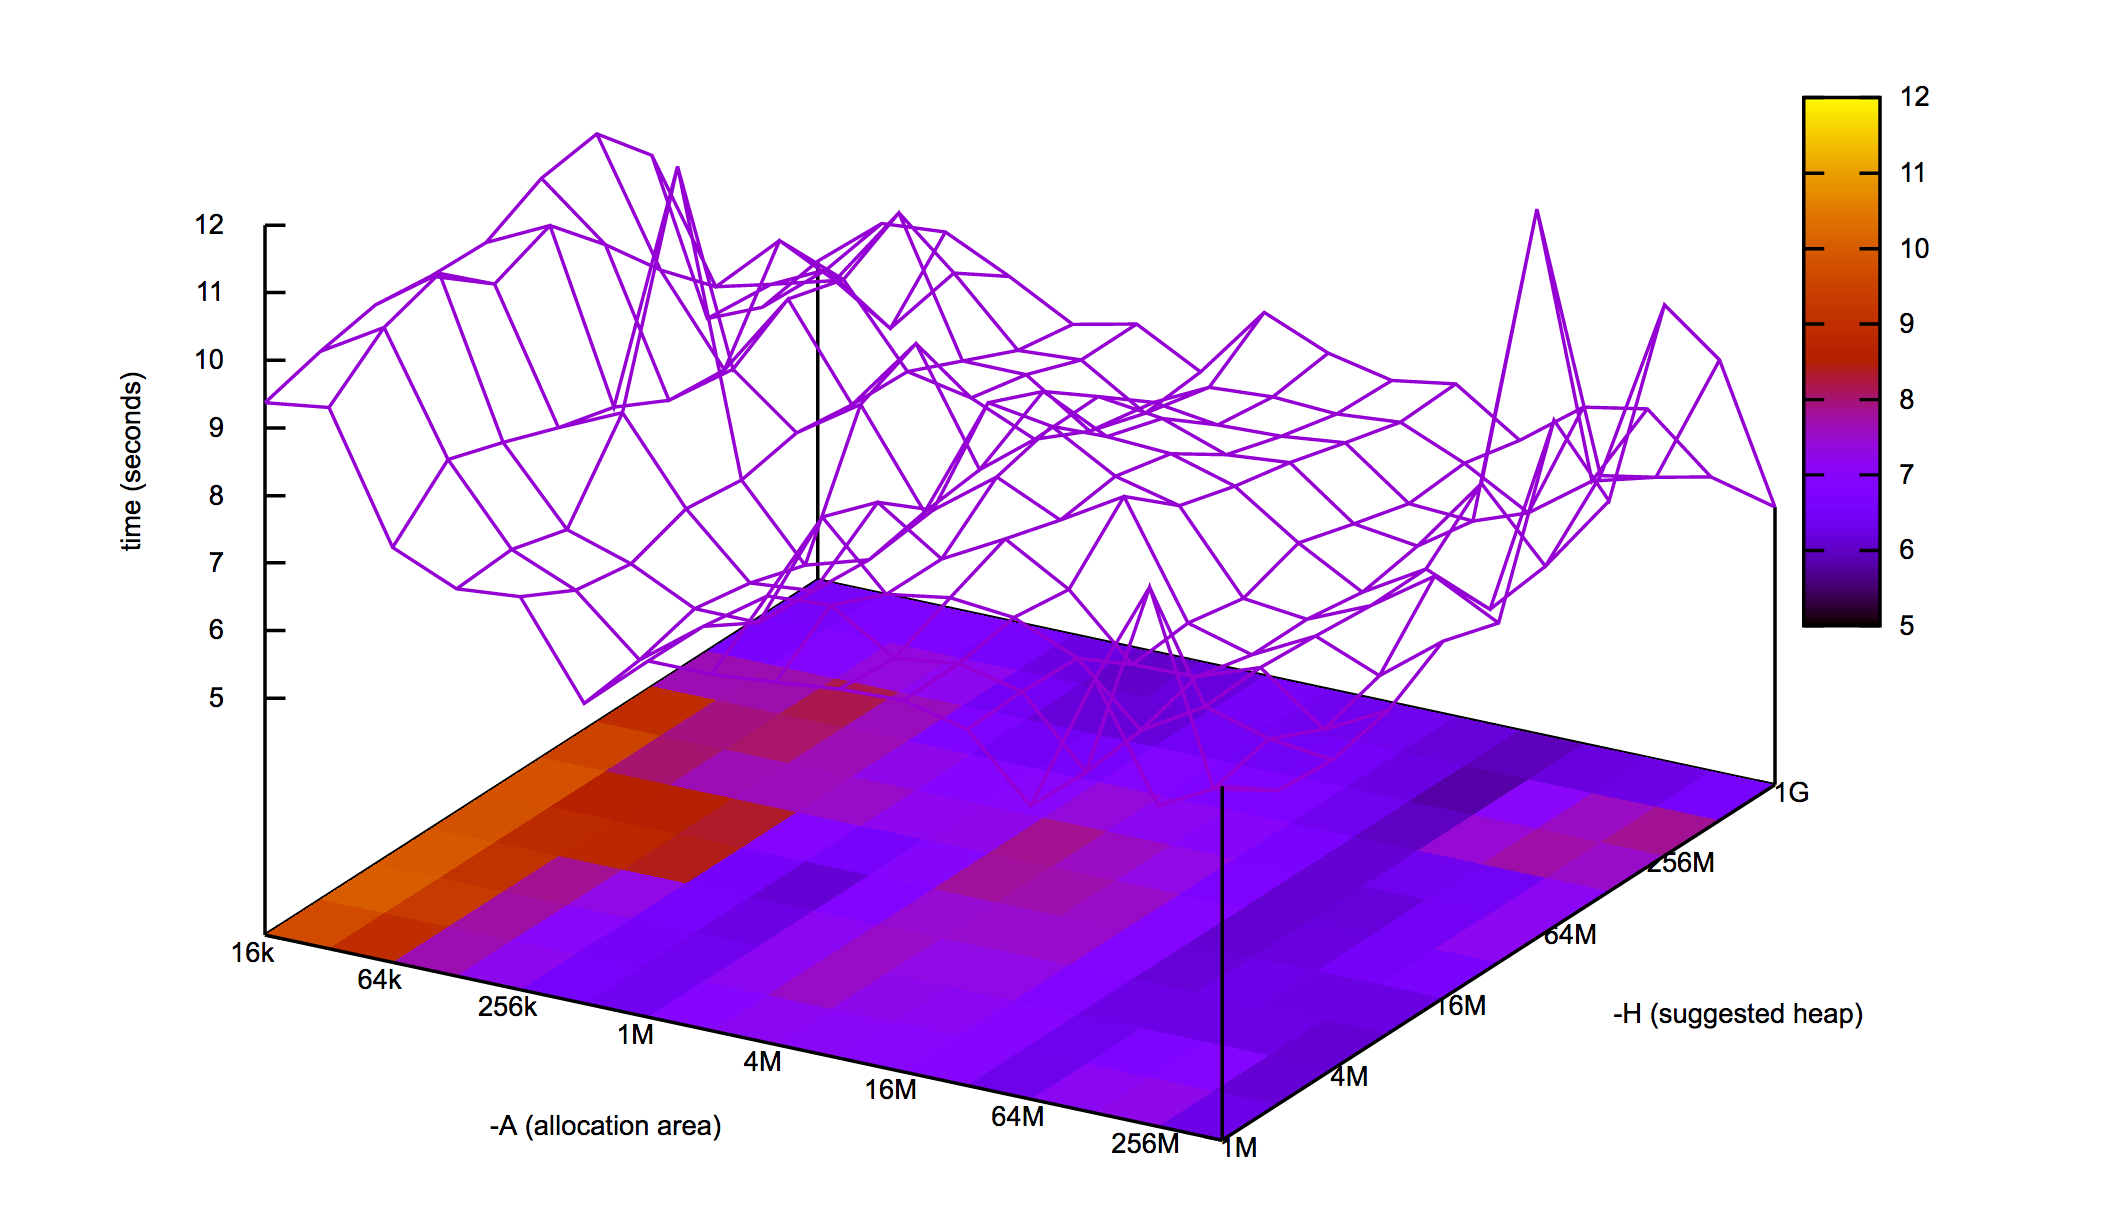
\includegraphics[width=\textwidth]{img/gc-tuning.png}
\caption{Garbage collection flags compared to execution time.}
\label{gc-tuning}
\end{figure}

Under some garbage collection settings, it is possible to improve the total
execution time in a 50\%. Without having to refactor the code, it is possible
to cut in half the time just by setting some options in the garbage collection.
\emph{Grasping to control, so I better hold on}. Although this results are
good, let us not be over-optimistic: by tuning this executable we may be making
the execution options specific to the problem that is being used, instead of
obtaining a general improvement. Over-fitting the
library to this concrete example is at risk.\\

To check if that is indeed the case, we can take a look at the general spectrum
of results generated by the tool (Figure \ref{gc-tuning}). In there, we can see
that the garbage collection settings are of great importance for the library:
in the plane that represents the different execution times, a flat shape would
indicate that there is not much influence done by the garbage collection. In
the plot we can see the opposite: a strenuous surface that represents the time
the execution expends on garbage collection, on how a difference in the
allocation space or heap available can increase up to a 40\% the total
computation time. In the results, there is an expected peak when the garbage
collection settings force the use of low memory, and its counterpart when the
settings are high. Although it may be tempting to offer the program the highest
memory flags to be sure of low execution times, this may be counter-productive
in lower-memory systems and parallel applications.\\


\subsubsection{Profiling different \texttt{PriorityQueue} implementations}

Now that we have discarded a substantial improvement by tuning with flags the
garbage collection, it's time to analyze the \texttt{PriorityQueue}
implementation and try to find if there is something to be improved in the
code. The code implements the priority queue over a package called
\texttt{heap}, which promises to deliver ``\textit{a flexible implementation of
  min-, max-, min-priority, max-priority and custom-priority heaps based on the
  leftist-heaps from Chris Okasaki's book Purely Functional Data Structures}''
\cite{okasaki-1999-purely}, which was exactly what was desired when
implementing the library (to follow the explanations in the literature).
However, this package may not be as suitable as thought for our purposes or it
may be a misuse of it. Running the \texttt{profiling} executable of the library
in this problem outputs, we can see these results (please bear in mind the
profiling overhead, stated as \texttt{PROF} time):\\

\begin{lstlisting}
> cabal run profiling
   4,452,597,512 bytes allocated in the heap
   5,673,545,840 bytes copied during GC
     234,847,840 bytes maximum residency (45 sample(s))
       1,616,992 bytes maximum slop
             472 MB total memory in use (0 MB lost due to fragmentation)

                                     Tot time (elapsed)  Avg pause  Max pause
  Gen  0      8573 colls,     0 par    1.030s   1.050s     0.0001s    0.0004s
  Gen  1        45 colls,     0 par    7.107s   7.359s     0.1635s    0.3832s

  TASKS: 4 (1 bound, 3 peak workers (3 total), using -N1)

  SPARKS: 0 (0 converted, 0 overflowed, 0 dud, 0 GC'd, 0 fizzled)

  INIT    time    0.001s  (  0.010s elapsed)
  MUT     time    3.333s  (  5.247s elapsed)
  GC      time    6.249s  (  6.495s elapsed)
  RP      time    0.000s  (  0.000s elapsed)
  PROF    time    1.888s  (  1.914s elapsed)
  EXIT    time    0.003s  (  0.046s elapsed)
  Total   time   11.475s  ( 11.797s elapsed)

  Alloc rate    1,335,764,960 bytes per MUT second

  Productivity  29.1% of total user, 28.6% of total elapsed
\end{lstlisting}


We can see how the profiler returns that only a 29.1\% of the time has been
spent in actual search computations, while more than half of the execution time
(54.5\%) has been spent in garbage collection. To check if this space leak is
caused by our implementation or by the library used to implement the priority
queue, we can experiment with different methods.\\

We can run the same problem using the implementation with the \texttt{psqueues}
(and more accurately the \texttt{Data.IntPSQ} module), an alternative library
that offers an implementation of a higher level than our original \texttt{heap}
package. The results are as follow:\\


\begin{lstlisting}
> cabal run profiling
   4,867,074,880 bytes allocated in the heap
   4,823,508,568 bytes copied during GC
     183,851,592 bytes maximum residency (46 sample(s))
       1,405,912 bytes maximum slop
             373 MB total memory in use (0 MB lost due to fragmentation)

                                     Tot time (elapsed)  Avg pause  Max pause
  Gen  0      9345 colls,     0 par    0.992s   1.017s     0.0001s    0.0018s
  Gen  1        46 colls,     0 par    5.654s   5.849s     0.1271s    0.2936s

  TASKS: 4 (1 bound, 3 peak workers (3 total), using -N1)

  SPARKS: 0 (0 converted, 0 overflowed, 0 dud, 0 GC'd, 0 fizzled)

  INIT    time    0.001s  (  0.012s elapsed)
  MUT     time    3.508s  (  4.884s elapsed)
  GC      time    5.292s  (  5.498s elapsed)
  RP      time    0.000s  (  0.000s elapsed)
  PROF    time    1.354s  (  1.367s elapsed)
  EXIT    time    0.003s  (  0.037s elapsed)
  Total   time   10.159s  ( 10.431s elapsed)

  Alloc rate    1,387,545,376 bytes per MUT second

  Productivity  34.6% of total user, 34.1% of total elapsed
\end{lstlisting}


There, it can be seen that the garbage collection time has been reduced by a
second, but it is still a marginal improvement. Therefore, maybe a different
approach is needed: If we take a close look to the \texttt{addList} method, the
main cost center of this problem, we can see that we have two main options to
implement it: the first of them is to create a new \texttt{MinPrioHeap} and use
the library function \texttt{union} to merge both of them inside the new
structure. The code is shown in the listing \ref{addlist:union}.\\

\begin{lstlisting}[style=haskell, caption= \texttt{addList} using
  \texttt{union}, label=addlist:union]
addList xs (PriorityQueue h f) = PriorityQueue (union h xs') f
  where xs' = fromList $ map (\n -> (f n, n)) xs
\end{lstlisting}

Although the language should manage the memory correctly, maybe this is not the
best way of managing this operation. As a possible solution, we can try to
force the reutilization of the old structure by adding the nodes using a strict
fold over the \texttt{MinPrioHeap}. This implementation is shown in the listing
\ref{addlist:fold}.\\

\begin{lstlisting}[style=haskell, caption= \texttt{addList} using
  \texttt{fold'}, label=addlist:fold]
addList xs (PriorityQueue h f) = PriorityQueue (foldl' insertNode h xs) f
  where insertNode acc x = insert (f x, x) acc
\end{lstlisting}

To check the performance of all possibilities, the profiling problem stated at
the beginning of this subsection has been run using all combination of
implementations and library, and the full results of performance are found in
the chart shown in the figure \ref{chart-libraries}.\\

\begin{figure}[ht]
  \centering
\begin{tikzpicture}
  \begin{axis}[
    xbar,
    y axis line style = { opacity = 0 },
    axis x line       = none,
    % width = 8cm, height = 4cm,
    ytick = data,
    xmin=0,
    tickwidth         = 0pt,
    enlarge y limits  = 1,
    enlarge x limits  = 0.02,
    symbolic y coords = {Package B,Package A},
    nodes near coords,
    ]
    \pgfplotsset{cycle list name=list}
  \addplot coordinates { (11.779,Package A) (11.046,Package B) };
  \addplot coordinates { (12.473,Package A) (10.677,Package B) };
  \legend{Using union, Using a fold}
  \end{axis}
\end{tikzpicture}
\vspace{-1cm}
\caption{Comparing Package A (\texttt{heap}) and Package B
  (\texttt{psqueues}).}
\label{chart-libraries}
\end{figure}

It can be seen how the performances are very similar to each other: no matter
which library or what implementation we use. We can then conclude that the
problem is intrinsic to the memory management performed by the RTS interface in
Haskell, or by how the compiler is turning the high-level declarations into
machine code.\\

Nonetheless, taking into account the knowledge that has been obtained by
profiling the data structure, the most intuitive and possible reason for this
space leak is that in Haskell, all data in immutable, and by adding the nodes
to the queue a complete new queue is being generated, allocating a new copy of
it and forcing the garbage collector to claim the old queue's space. Although
this is the natural behavior expected from the language, there are workarounds
to make a data structure mutable, but it has been impossible to find an
implementation that allows for a low complexity insertion and extraction of
nodes in a sorted heap and that is mutable. Implementing such data structure in
Haskell is not an easy task, and it is considered to be out of the scope of
this thesis.\\

\newpage

%%% Local Variables:
%%% TeX-master: "tfg"
%%% End:
\section{Project Organization \& Management}

\subsection{Planning}

\subsubsection{Time Management}

For a project of this size, it is important to develop a plan that states
different stages. In Figure \ref{gantt} it is possible to see a Gantt project
that sums the project planning for a complete year.\\

\begin{figure}[ht]
  \centering
  \begin{ganttchart}[vgrid = dotted, hgrid = dotted, compress calendar,
    time slot format=isodate-yearmonth, x unit = 8mm,
    group left shift = 0.1, group right shift = -0.1,
    title/.append style={fill=azulUC3M, draw=white, thick},
    title label font=\color{white}\ttfamily,
    title height = 1,
    group/.append style={fill=azulUC3M},
    group label font = \small,
    bar/.append style={fill=azulUC3M, draw=none, rounded corners=3pt},
    bar label font = \small,
    milestone/.append style={draw=azulUC3M, fill=azulUC3M},
    milestone label font = \small,
    link/.append style={azulUC3M}]
    {2016-09}{2017-09}
    \gantttitlecalendar{year, month} \\
    
    \ganttgroup{Phases}{2016-09}{2017-02}
    \ganttgroup{}{2017-03}{2017-06}
    \ganttgroup{}{2017-07}{2017-09} \\

    % \ganttgroup{Research}{2016-09}{2017-06} \\
    \ganttbar{Previous Research}{2016-09}{2016-10} \\
    \ganttlinkedbar{Analysis}{2016-10}{2016-11} \\
    \ganttlinkedbar{Design \& Modelling}{2016-12}{2017-02} \\ 
    \ganttlinkedmilestone{Initial design}{2017-02} \\
    
    % \ganttgroup{Development}{2017-03}{2017-09} \\
    \ganttlinkedbar{Implementation}{2017-03}{2017-05} \\
    \ganttlinkedbar{Testing}{2017-04}{2017-06} \\
    \ganttlinkedmilestone{\texttt{v0.1.0.0}}{2017-06} \\
    
    % \ganttgroup{Testing}{2017-07}{2017-09} \\
    \ganttlinkedbar{Iteration}{2017-07}{2017-08} \\
    \ganttlinkedmilestone{\texttt{v0.2.0.0}}{2017-08}
    \end{ganttchart}
  \caption{Gantt chart for the project.}
  \label{gantt}
\end{figure}

In the chart, it is possible to observe that there have been three main
milestones in the project:

\begin{itemize}
\item \textbf{The initial design}: A complete design of the interface, with a
  provisional type definition set. This implies that the requirements and use
  cases have already been studied, and the research and analysis phases have
  been completed already. This design is not final and immutable, of course:
  it serves as a guideline for the implementation and requirement tracking.
\item \textbf{Version 0.1.0.0}: The first version of the library. Lacking
  several features, it includes a set of algorithms to be imported that have
  been tested and proved correctly.
\item \textbf{Version 0.2.0.0}: The final version of the project assigned to
  this thesis; includes all the algorithms mentioned in this document and
  benchmarking tools.
\end{itemize}

It is also important to clarify that the ``Implementation'' tasks imply more
than simply writing the code needed: along with it, all the documentation have
to be appropriately written and updated as the codebase evolves. In the
``Testing'' tasks is also included all the required benchmarking to ensure the
correctness of the algorithms. The task of ``Iteration'' is vaguely defined on
purpose: depending on the evolution of the project, this may consist on further
improvements or testing to complete the features and requirements in this
document.\\

\subsubsection{Version Control \& Continuous Integration}

To manage all the code in the project, it is a must to use a Version Control
System (VCS). The chosen system for the project is Git, a widespread
distributed VCS that allows us to keep track of all changes in the code in all
developing devices as well as in a remote server \cite{chacon-2009-git}. The
way Git works allows us to maintain all the code in the repository and enables
different collaboration dynamics that will be required for the open release of
the project.\\

One of the main features of Git is the branching system: a repository contains
one main branch (\texttt{master}), which contains all the commits (snapshots
that include all code at a certain point in time in the project) associated
with it. The users can create a new branch from it, to add new features or try
new implementations, and merge back the changes when satisfied or keep on
creating new branches on it. This system allows a great flexibility, which can
sometimes become a problem; for that reason some workflows have been designed
to impose some restrictions to Git usage in big projects that are maintained by
several developers. For this project, the choice used is a slight modification
of Git-flow \cite{driessen-2010-gitflow}, that uses the \texttt{master} branch
as the branch where \texttt{HEAD} represents the last delivered development
changes. In the original workflow proposed, this branch is only for
production-ready code, but the author considers this redundant and in the
project repository it is stated that the production-ready code is the one
tagged as releases in the repository \cite{chacon-2009-git}, and distributed in
the Haskell package managers available. All support branches should be branched
from \texttt{master} and merged back into it once the code is ready, as stated
in the \texttt{CONTRIBUTING} file.\\

However, we also must define what ``ready'' actually means: to do so, we will
rely in one of the tools provided by the third-party service that hosts the
code: GitLab, which offers the possibility of configuring different Continuous
Integration tasks and pipelines. Continuous Integration is the practice of
merging often the developer copies of the project into the main repository
\cite{fowler-2006-ci}, and the tools provided by the service allows us to run
some code on the server side and return some insights. In this particular case,
the pipeline configured installs a Docker image containing Haskell, installs
and builds the project and then runs the tests defined in the project's test
suite. This configuration is stored in the file \texttt{.gitlab-ci.yaml} and
can be read in Listing \ref{git-ci}.\\

\begin{lstlisting}[label=git-ci,
caption=Continuous Integration pipeline configuration]
image: haskell:8.0

before_script:
  - cabal update
  - cabal install --only-dependencies --enable-tests

test:
  script:
  - cabal configure --enable-tests
  - cabal build
  - cabal test
\end{lstlisting}

If the project can install all dependencies, be compiled and run all tests
without failures, the commit gets tagged as ``passed''. If not, the build is
considered to fail and an email notification gets sent to the collaborator that
pushed the code to the repository. Only passed pull-requests can be merged into
master, forcing the work-in-progress to stay in the adequate branch and the
code to be ready before be merged into the master branch.\\

\subsection{Budget}

For this project, the budget is divided in two main categories:

\begin{itemize}
\item \textbf{Direct costs}: all the personal costs along with the value of the
  equipment used during the project.
\item \textbf{Indirect costs}: which are not related to production and cannot
  be accounted to an object or staff member. For the project, these costs have
  been decided to be fixed on a 10\% of the direct costs.
\end{itemize}

Although the staff of this project has been formed by a single person, we can
differentiate between several positions.\\

\begin{table}[!htbp]
   \centering
   \rowcolors{2}{gray90}{white}
   \begin{tabular}{| l | r | r | r |}
     \hline
     Position & \euro / Hour & Hours invested & Cost \\
     \hline
     Project Manager & 25 & 150 & 3750 \euro \\
     Developer       & 15 & 200 & 3000 \euro \\
     Q \& A          & 10 & 50  & 500  \euro \\
     \hline
     \multicolumn{3}{| l |}{Total}  & 7250 \euro \\
     \hline
   \end{tabular}
   \caption{Personnel costs}
   \label{bg:staff}
\end{table}

Apart from these costs, it is also important to compute the imputable costs for
the hardware and software used during this project. It is important to notice
that this project has a time span of 12 months, since that is a key factor to
compute the imputable costs for each item.\\

\begin{table}[!htbp]
   \centering
   \rowcolors{2}{gray90}{white}
   \begin{tabular}{| l | r | r | r |}
     \hline
     Item & Total Price & Life Span  & Imputable Cost \\
     \hline
     MacBook Pro (Retina, 13-inch)  & 1524.64 \euro & 48 months & 381.17 \euro \\
     GitLab Enterprise Edition      & 13.79 \euro   &  1 month  & 165.48 \euro \\
     \hline
     \multicolumn{3}{| l |}{Total}  & 546.65 \euro \\
     \hline
   \end{tabular}
   \caption{Equipment costs}
   \label{bg:equip}
\end{table}

Using these two costs it is possible to compute the complete budget for the
project. The final amount consists in the sum of this costs plus a 10\% of that
amount to cover the indirect costs. \\

\begin{table}[!htbp]
   \centering
   \rowcolors{2}{gray90}{white}
   \begin{tabular}{| l | r |}
     \hline
     Concept & Total \\
     \hline
     Personnel Costs & 7250 \euro \\
     Equipment Costs & 546.65 \euro \\
     Indirect Costs  & 779.97 \euro \\
     \hline
     \textbf{Project Costs}  & \textbf{8579.62 \euro} \\
     \hline
   \end{tabular}
   \caption{Total project costs}
   \label{bg:total}
\end{table}

In Table \ref{bg:total} is possible to see that the total costs sum up to
8579.62 \euro for the project. The final project budget is that amount, plus
the fixed percentages of risk (estimation of the money that may be needed due
to unexpected events) and benefits (value generated in the project). Estimating
both percentages at 10\%, we obtain 857,96 \euro benefits and a \textbf{total
  project budget of 10295.54 \euro}. \\

\subsection{Open-Sourcing the Project}

\subsubsection{License \& Legal Framework}

Making the project open source requires a deep research of the available
distribution licenses for this type of works. To be able to choose the adequate
license, first it is needed to state the objectives of the project: What are the
goals trying to be achieved? Once the target is well defined, it will be an
easy task to choose an adequate license from the ones available
\cite{morin-2012-license}.\\

When making this project open source, the main goal in this project is
for it to be improved and peer-reviewed by potential users and contributors.
Although the project is right now a functional piece of software, the
complexity of techniques in the software and elaborate abstractions used in
Haskell leave a great room for improvement: a cleaner code and a greater
performance can still be obtained. Apart from improving the present state of
the code, the adding of new features by some users can be interesting, like
algorithms or automation features for the framework. For that reason, the
license needs to be flexible for the user while ensuring transparency and a
completely open development.\\

Following these characteristics, the most adequate license found for the
project is the GNU General Public License v3.0, which ensures that the code is
open and free, and all variations of it are forced to maintain this status.
This will help the project take advantage of any feedback in derivatives as
well as spreading the open-nature of this license. This license provides
reasonable constraints for businesses as well as appropriate perks for
education: commercial use, distribution, modification, patent use, and private
use are allowed as long as the source code is disclosed, licensed under the
same license and the changes performed are stated. This license also provides
no liability or warranty with the software.\\

\subsubsection{Contribution Workflow}

Since the project aims to attract users to contribute, it is considered a good
practice to offer some contribution guidelines for interested users to follow.
This guidelines are collected in the file \texttt{CONTRIBUTING} and gather all
the steps to have homogeneous code and methodologies throughout the whole
project. In this section, this guidelines will be explained on detail.\\

First, the user is asked to create a new issue in the remote repository
provider, GitLab. This prevents two users to start working on clashing or
redundant tasks and offers a better perspective when organizing the project.
Some guidelines are also given when forking or branching (following the scheme
specified before for branching/merging). There is a special emphasis on test
creation: this will prevent future refactors or improvements to break previous
features. Once the contribution is ready on a forked version of the repository,
a pull-request can be performed. This will no automatically merge the code, but
instead it will start a code review process. This code review will ensure that
the code has been developed following the guidelines mentioned, and will enable
feedback from the project maintainer(s) to the user in order to create better,
more adequate code for the project \cite{beller-2014-review}. Once the code
review has been approved, the code is merged to the main code and only accepted
in the repository if all the Continuous Integration stages (install
dependencies, building and testing) are properly completed.\\

\newpage

%%% Local Variables:
%%% TeX-master: "tfg"
%%% End:

\section{Conclusions}

The main purpose of the thesis was to create a framework for designing,
developing and testing search algorithms in a purely functional environment
like Haskell. In spite of the pitfalls found, the author thinks that the
objective has been accomplished.\\

Agis will be published as a Haskell package and open sourced to enable further
development. The main codebase contains a set of algorithms ready to solve
search problems, but it also provides several parts of search algorithms
already implemented and ready to be included in user-designed algorithms: for
instance, a node expansion function. This pieces are general enough to provide
flexibility to the user for their own designs. A set of types is defined in the
library with a comprehensive documentation, for the user to understand
correctly all the inputs and outputs for each function, and make all the pieces
fit in the library. These types enable the user's algorithm to be treated just
like a library algorithm: that means that all the algorithms can be used to
solve the same problems in the same way, and can be tested and benchmarked in
the same manner.\\

The set of algorithms provided by the library include some of the best known
algorithms, that have been implemented following a closed list per node (that
enables the search for the $k$ best solutions). This affects performance in
some cases, but can yield some interesting insight when used for educational
purposes. It is important to notice that this approach (the fact of providing
the $k$ best solution algorithms instead of classical, single solution
algorithms) was created in the research and analysis phase, where it appeared
as an incredibly intuitive option to solve the closed list problems. Haskell's
laziness and ability to deal with infinite sets of data turned out to provide a
clean and elegant solution to this problem, that was worth to work on. That is
indeed a hands-down conclusion of the project: when used for clear, state-less
computation; Haskell provides a clean syntax, with almost no noise or verbosity
(although it might seem obscure for some programmers if used to a more
traditional, imperative syntax).\\

However, Haskell also provides a great set of tools for input and output, that
are able to isolate the side-effects of the computations. When this is combined
with the vast community after Haskell, the results are great, high-level
packages that deal with the side effects in a concise way; being a great
example of that the \texttt{criterion} package used for the benchmarks in this
project. It offers one-liner functions that allow to launch several-iterations
of timings and prints all the important data of those timings.\\

But a key feature and motivation behind this project is that Haskell's purity
provides pure parallelism: all the pure code (which, simplifying it, is all the
code without \texttt{IO} types) is able to trivially support parallelism by
enabling a compiler flag. Pure parallelism enabled by GHC is guaranteed to be
deterministic and not to have any race conditions or deadlocks \cite{ghc}. The
fact of being able to build a complete framework for heuristic search works
using purely functional programming brings that advantage, that can be
incredibly useful in the future following the current trends.\\

% Also important in these project was the organization. This was the biggest
% project developed by the author, and it would not be possible without a
% planning like the one developed for this project. Although the times were not
% uniform as it could be (due to the rest of academic duties), the milestones
% stated in the planning were respected and delivered on time, so the project
% could go on without any late deliveries.\\

As a summary of personal conclusions of the author, the new insight provided by
this translation of typical search algorithms to a new paradigm is priceless.
Along with it, the experience gained through this months in a different
framework that the one used in the courses of the university was an interesting
effort that provided several mechanisms and paradigms that can be exported to
other languages. Although Haskell has been typically overlooked by the industry
in favor to other languages, the functional programming paradigm is an upward
trend that seem to bring some key concepts to our current development and
progress.\\

\newpage

%%% Local Variables:
%%% TeX-master: "tfg"
%%% End:
\section{Future Work}

\newpage

%%% Local Variables:
%%% TeX-master: "tfg"
%%% End:

\begin{appendices}

\section{Documentation}

This appendix includes a PDF version of the documentation for the library. This
documentation is generated by Cabal using the \texttt{haddock} tool. Its LaTeX
backend is, however, deprecated; so this document has been generated as a PDF
from the HTML documentation available online for the library. The reason for
this clarification is to beware warn the reader and apologize for any possible
graphical artifacts that may have been included in this process.\\

The documentation includes the comprehensive description of all the functions
provided in all the modules of the package, being them described in
alphabetical order. This order is the one followed in the library index as
well, that may serve as a possible reference. If the reader is using a PDF
version of this thesis, please notice that all the hyperlinks were dropped in
the conversion to the adequate format, and it is recommended to check the
online version of the documentation for ease of use.\\

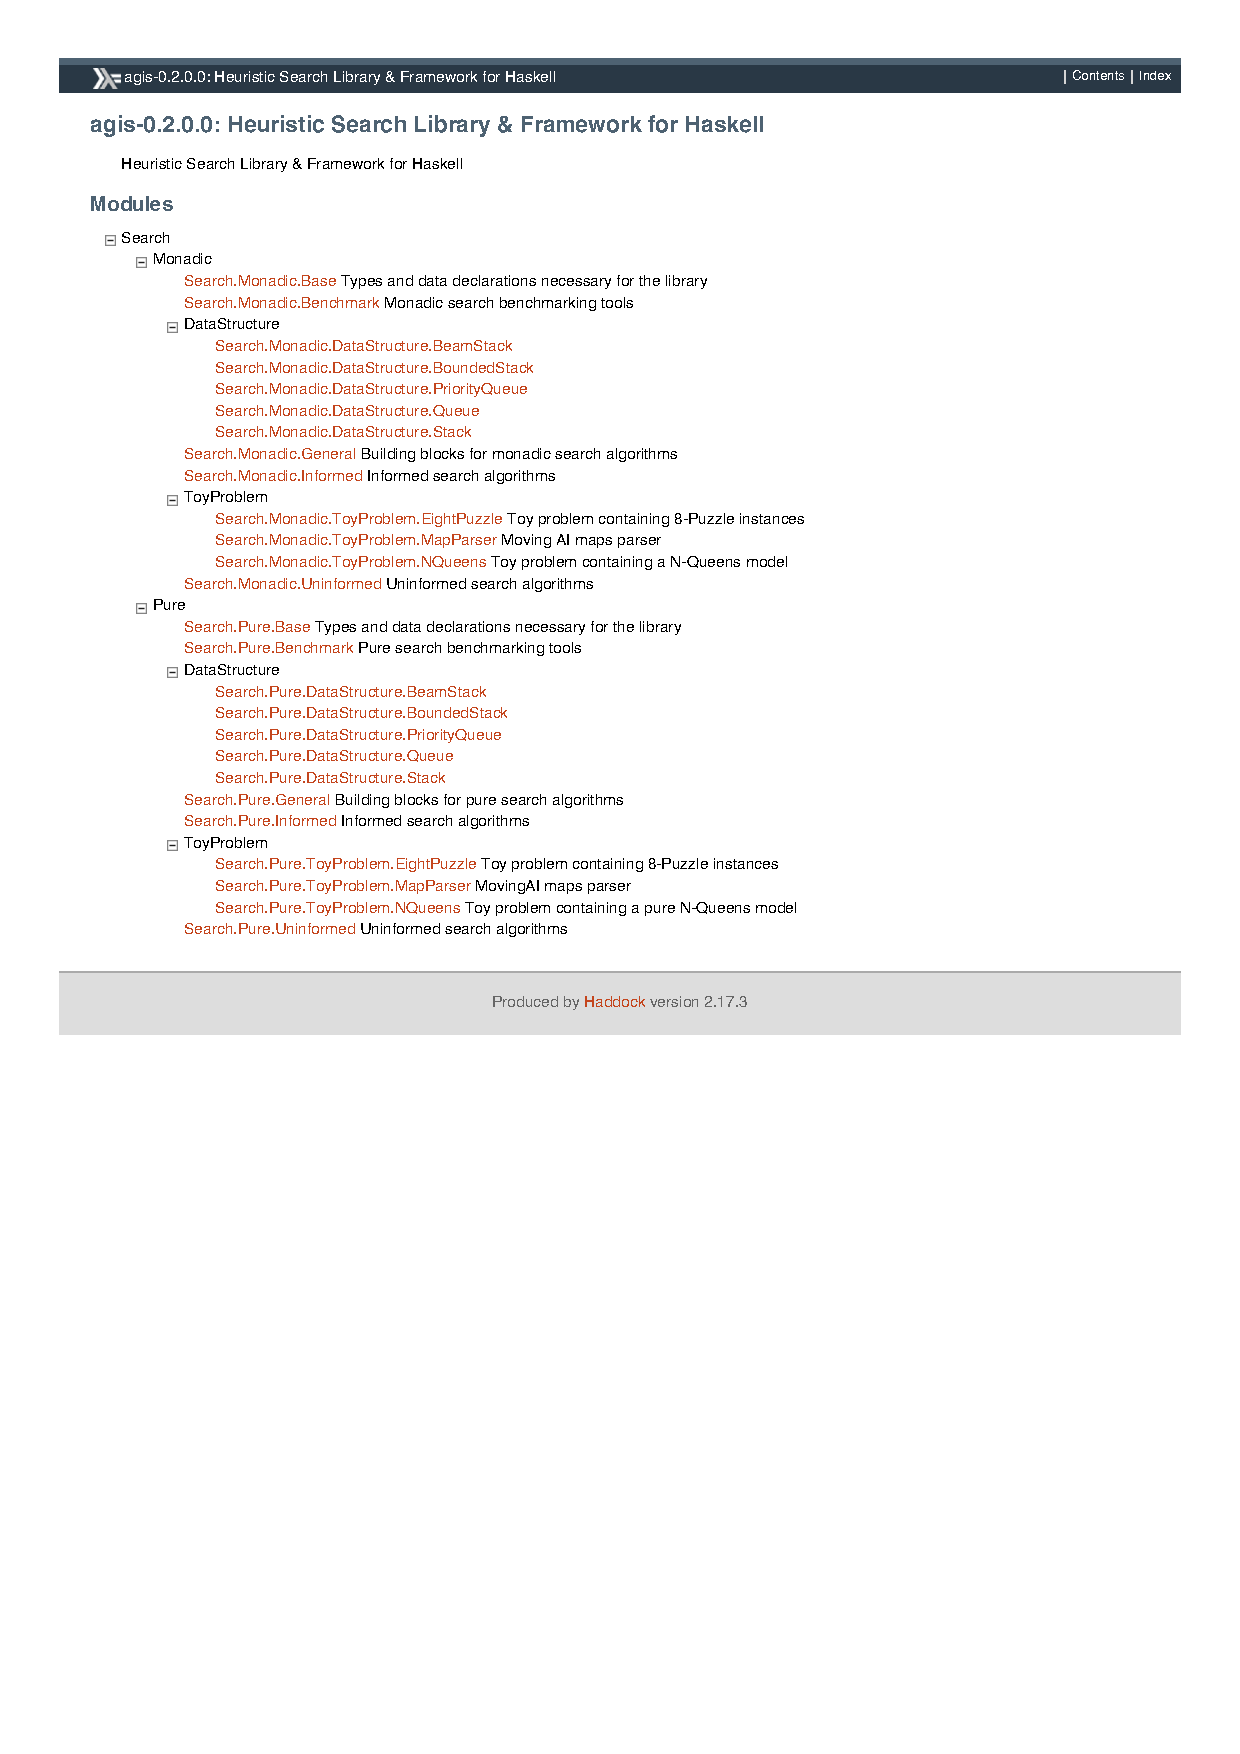
\includepdf[pages=-]{docs.pdf}

\end{appendices}
%%% Local Variables:
%%% mode: latex
%%% TeX-master: "tfg"
%%% End:


\clearpage

\addcontentsline{toc}{section}{References}
\bibliographystyle{apalike}
\bibliography{refs}

\end{document}
